\documentclass{elsarticle} 
\usepackage{url}
\usepackage{color,graphicx}
\usepackage{abstract}
\usepackage{enumerate}
\usepackage{amssymb,amsmath,amsthm}
\usepackage[numbers]{natbib}
\usepackage{booktabs}

%%%Need to include this code bit so that manuscript.tex can be made
%%%according to elsevier specs
\makeatletter\ifx\SetFigFont\undefined%
\gdef\SetFigFont#1#2#3#4#5{%
  \reset@font\fontsize{#1}{#2pt}%
  \fontfamily{#3}\fontseries{#4}\fontshape{#5}%
  \selectfont}%
\fi%


%%% Environment for notation and a symbol command to go along with it.
%%% The argument should be the widest symbol which is expected if 
%%% \sym will be used to make the list.
%%%
\newenvironment{notation}[1]{%
\begin{list}{}{\small
\settowidth{\labelwidth}{{#1}\quad}%
\setlength{\itemsep}{1.5pt plus 0.5pt minus 0.2pt}%
\setlength{\parsep}{0ex}%
\setlength{\rightmargin}{0em}%
\setlength{\leftmargin}{\labelwidth}%
\addtolength{\leftmargin}{\labelsep}%
\addtolength{\leftmargin}{1em}}}{\end{list}}

\newcommand{\sym}[1]{\item[${#1}$\hfill{}]}

\newcommand{\bx}{\mathbf{x}}
\newcommand{\bu}{\mathbf{u}}
\newcommand{\bd}{\mathbf{d}}
\newcommand{\til}[1]{\tilde{#1}}
\newcommand{\norm}[1]{\vert #1 \vert}
\newcommand{\set}[1]{\left\lbrace #1 \right\rbrace}
\newcommand{\SetAlgoLined}{}

\newcommand{\I}{\mathcal{I}}
\newcommand{\BO}{\textrm{BO}}
\newcommand{\IP}{\textrm{Ip}}
\newcommand{\UP}{\textrm{Up}}
\newcommand{\DN}{\textrm{Dn}}
\newcommand{\Inv}{\textrm{Iv}}
\newcommand{\Dem}{\textrm{Dm}}
\newcommand{\ulambda}{\underline{\lambda}}
\newcommand{\olambda}{\overline{\lambda}}
\newcommand{\eig}{\text{eig}}
\newcommand{\diag}{\text{diag}}


\newtheorem{theorem}{Theorem}
\newtheorem{lemma}[theorem]{Lemma}
\newtheorem{proposition}[theorem]{Proposition}
\newtheorem{conjecture}[theorem]{Conjecture}
\newtheorem{corollary}[theorem]{Corollary}

\theoremstyle{definition}
\newtheorem{definition}[theorem]{Definition}
\newtheorem{remark}[theorem]{Remark}
\newtheorem{assumption}[theorem]{Assumption}
\newtheorem{hypothesis}[theorem]{Hypothesis}
\newtheorem{property}[theorem]{Property}



\title{Economic model predictive control for inventory management in
    supply chains}
\author{Kaushik Subramanian, James B. Rawlings \corref{cor1}} \author
       {Christos T. Maravelias}
\address{Department of Chemical and Biological Engineering, University
  of Wisconsin-Madison, U.S.A.}
\cortext[cor1]{Corresponding author: rawlings@engr.wisc.edu}


\begin{document}
\begin{abstract}
  In this paper, we propose economic model predictive control 
 with guaranteed closed-loop properties for supply chain optimization. We
  propose a new multiobjective stage cost that captures economics as
  well as risk at a node, using a weighted sum of an economic cost and
  a tracking stage cost. We also demonstrate integration of scheduling
  with control using a supply chain example. We integrate a scheduling
  model for a multiproduct batch plant with a control model for
  inventory control in a supply chain. We show recursive feasibility
  of such integrated control problems by developing simple terminal
  conditions.
\end{abstract}
\begin{keyword} economic model predictive control \sep supply chain
  optimization \sep inventory control \sep scheduling
\end{keyword}
\maketitle
\section{Introduction}
Control theory for inventory management in supply chains is an
important area of research
\cite{sarimevis:patrinos:tarantilis:kiranoudis:2008,
  ortega:lin:2004}. Over the past decade, rolling
horizon optimization for inventory management has been studied \cite{perealopez:ydstie:grossmann:2003,mestan:turkay:arkun:2006,dunbar:desa:2007a,seferlis:giannelos:2004, kempf:2004,braun:rivera:flores:carlyle:kempf:2003,Maestre:Pena:Camacho:2009,maestre:pena:camacho:2011}. An
important consideration in process control is the stability of the
closed-loop under the proposed control. In
\cite{lin:wong:jang:shieh:chu:2004, venkateswaran:son:2005,
  hoberg:bradley:thonemann:2007}, the closed-loop stability for
classical control theory applied to inventory management was
studied. However, the stability of rolling horizon optimization
methods for inventory management has not been studied extensively.
%While closed-loop stability
%has been investigated for inventory control using classical control
%theory
%\cite{lin:wong:jang:shieh:chu:2004,venkateswaran:son:2005,hoberg:bradley:thonemann:2007},
%the stability of rolling horizon optimization based control methods
%for supply chains has not been studied extensively.  
Model Predictive
Control (MPC) is a rolling horizon optimization based control
algorithm with guaranteed stability properties.
Although, stability theory for MPC is a fairly mature field
\cite{rawlings:mayne:2009}, most 
implementations of MPC for supply chain do not consider stability. In
\cite{subramanian:rawlings:maravelias:2013}, we proposed centralized
and cooperative MPC with stability and asymptotic convergence
guarantees for a supply chain tracking inventories to its
setpoint. Our focus in this paper is to use recent developments in 
Economic MPC \cite{amrit:rawlings:angeli:2011,
  diehl:amrit:rawlings:2011} to develop a closed-loop stable model
predictive controller for supply chains in which we directly optimize
the economic cost of operating the supply chain.

This paper is organized as follows. In Section \ref{sec:ecoMPC}, we
briefly describe the main results of Economic MPC. In Section
\ref{sec:model}, we derive the state space model for a two-node supply
chain. In Section \ref{sec:ecoMPC_res}, we show the results for
economic MPC on a simple two-node supply chain. In Section
\ref{sec:multiobj}, we propose a novel
multiobjective MPC formulation that accounts for supply chain
economics as well as risk. In Section \ref{sec:multi} we implement MPC for a 
multiechelon, multiproduct supply chain example. In Section
\ref{sec:multi:integration}, we use periodic terminal condition ideas from
\cite{subramanian:maravelias:rawlings:2012} to integrate scheduling
with inventory control. Finally, we present our conclusions in Section
\ref{sec:conclusions}.

\section{Economic MPC}
\paragraph{Note} We only state important Economic MPC stability results in this section. The interested reader can refer to \cite{amrit:rawlings:angeli:2011,
  diehl:amrit:rawlings:2011} for details.
\label{sec:ecoMPC}
\paragraph{Model.}
We consider the following linear model
\begin{equation}
\label{eq:model}
x^+ = Ax + Bu + B_dd
\end{equation}
in which $x \in \mathbb{R}^n$ is the system state, $u \in
\mathbb{R}^m$  is the manipulated input and $d \in \mathbb{R}^d$ is
the disturbance to the system. We develop economic MPC theory for
the nominal disturbance, denoted by $d_s$. We assume that the system
$(A,B)$ is stabilizable.

\paragraph{Constraints.}
The states and inputs are constrained as follows:
\begin{equation}
x \in \mathbb{X} \qquad u \in \mathbb{U}
\end{equation}
\paragraph{Stage cost.}
The economic cost for implementing input $u$ from state $x$ is given
by $\ell(x,u)$. 
\paragraph{Optimal steady state.}
We define the steady-state problem for the nominal demand $d_s$ as follows:
\begin{equation}
\label{eq:SS}
\min_{x,u}{\ell(x,u)} \qquad \text{s.t.~} x = Ax + Bu + B_dd_s, \quad x \in
\mathbb{X}, u \in \mathbb{U}
\end{equation}
The optimal steady state is denoted by $(x_s,u_s;d_s)$

We make the following assumptions:
\begin{assumption}
\label{ass:closed}
The constraint set $\mathbb{X}$ is convex and  closed. The constraint set
$\mathbb{U}$ is convex and compact. The optimal steady state $(x_s,u_s;d_s)$
is such that $x_s \in \mathbb{X}$ and $u_s \in \mathbb{U}$
\end{assumption}

\begin{assumption}
\label{ass:strict_dissipativity}
There exists $(x_s,u_s;d_s)$ and $\lambda_s$ so that 
\begin{enumerate}[(a)]
\item $(x_s,u_s;d_s)$  is a unique solution of \eqref{eq:SS}.
\item The multiplier $\lambda_s$ is such that $(x_s,u_s;d_s)$
  uniquely solves \eqref{eq:SS1}
\begin{equation}
\label{eq:SS1}
\min_{x,u}{\ell(x,u)+\lambda_s'[x-(Ax+Bu+B_dd_s)]} \quad \text{s.t.~}
  x \in \mathbb{X}, u \in \mathbb{U}
\end{equation}
\item The system $x^+=Ax+Bu+B_dd_s$ is strictly dissipative with respect
  to the supply rate $s(x,u) = \ell(x,u)-\ell(x_s,u_s)$ and
  storage function $\lambda(x) = \lambda_s'x$. That is, there exists a
  positive definite function $\rho(\cdot)$ such that
for all $(x,u) \in \mathbb{X} \times \mathbb{U}$
\begin{equation}
\label{eq:esc:strict_dissipativity}
\lambda_s'(Ax+Bu+B_dd_s-x) \leq -\rho (x-x_s)+s(x,u)
\end{equation}
\end{enumerate}
\end{assumption}

\begin{assumption}[Basic stability assumption]
\label{ass:bsa}
There exists a convex, compact terminal region $\mathbb{X}_f \subseteq
\mathbb{X}$, containing the point $x_s$  and a control
law $\kappa_f: \mathbb{X}_f \rightarrow \mathbb{U}$  and a function
$V_f:\mathbb{X}_f \rightarrow \mathbb{R}$ such that the
following holds for all $x \in \mathbb{X}_f$
\begin{align}
\label{eq:BSA}
&V_f(Ax+B\kappa_f(x)+B_dd_s) \leq V_f(x)-\ell(x,\kappa_f(x))+\ell(x_s,u_s) \\
\label{eq:esc:invariant}
&Ax+ B\kappa_f(x) +B_dd_s \in \mathbb{X}_f
\end{align}
\end{assumption}

We first define the terminal constraint MPC problem
\begin{xalignat}{2}
\label{eq:PN_equality}
\mathbb{P}_N(x;d_s) :& \min_{\bu}{V_N(\bu;x)} & \nonumber \\
&\text{s.t.~} x(0) = x \nonumber & \\
&x(j+1) = Ax(j) + Bu(j) +B_dd_s, & j \in
\mathbb{I}_{0:N-1} \nonumber \\
&x(j) \in \mathbb{X}& j \in \mathbb{I}_{0:N-1} \\
&u(j) \in \mathbb{U}& j \in \mathbb{I}_{0:N-1} \nonumber \\
&x(N) = x_s & \nonumber
\end{xalignat}
in which the cost function $V_N(\bu;x)$ is the sum of stage
costs
\begin{equation}
\label{eq:VN_equality}
V_N(\bu;x) = \sum_{j=0}^{N-1} \ell(x(j),u(j)) 
\end{equation}
The control horizon is denoted by $N$, the input sequence $\bu =
(u(0),u(1),\ldots,u(N-1))$ and the symbol $\mathbb{I}_{k:l}$ stands
for the set $\set{k,k+1,\ldots,l}$.

The control law $\kappa(x)$ is the first input in the optimal
solution $\bu^0(x)$ to optimization problem
\eqref{eq:PN_equality}. The admissible region $\mathcal{X}_N$ is
given by
\[ \mathcal{X}_N := \set{ x \in \mathbb{X} \mid \exists \bu \in
  \mathbb{U}^N, \text{ s.t. \eqref{eq:PN_equality} is feasible}}
\]
The following is the exponential stability theorem for economic MPC
that solves problem \eqref{eq:PN_equality} online
\citep{diehl:amrit:rawlings:2011}.  

\begin{theorem}[Lyapunov function with terminal constraint]
\label{thm:equality}
Let the system $(A,B)$ be stabilizable. Let Assumptions \ref{ass:closed} and \ref{ass:strict_dissipativity}
hold. Then the steady-state solution of the closed-loop system $x^+ =
Ax+B\kappa(x)+B_dd_s$ is asymptotically stable with
$\mathcal{X}_{N}$ as the region of attraction. The Lyapunov function
is
\[ \tilde{V}(x) := V_N^0(x) +\lambda_s'[x-x_s]-N\ell(x_s,u_s) \]
in which $V_N^0(x)$ is the optimal cost function of \eqref{eq:PN_equality}
\end{theorem}

We  also define the terminal region/penalty MPC problem as follows:
\begin{xalignat}{2}
\label{eq:PN_region}
\mathbb{P}_N(x;d_s) :& \min_{\bu}{V_N(\bu;x)} & \nonumber \\
&\text{s.t.~} x(j+1) = Ax(j) + Bu(j) +B_dd_s, & j \in
\mathbb{I}_{0:N-1} \nonumber \\
&x(j) \in \mathbb{X}& j \in \mathbb{I}_{0:N-1} \\
&u(j) \in \mathbb{U}& j \in \mathbb{I}_{0:N-1} \nonumber \\
&x(N) \in \mathbb{X}_f & \nonumber
\end{xalignat}
in which the cost function $V_N(\bu;x)$ is 
\begin{equation}
\label{eq:VN_region}
V_N(\bu;x) = \sum_{j=0}^{N-1} \ell(x(j),u(j)) + V_f(x(N))
\end{equation}
Note that in contrast to objective function  \eqref{eq:VN_equality}, we modify the
cost function in the terminal penalty formulation by adding a
terminal penalty $V_f(x(N))$. Similarly, in the optimization problem
\eqref{eq:PN_region}, the terminal constraint is
replaced by the terminal region. The terminal region $\mathbb{X}_f$
and the terminal penalty $V_f(\cdot)$ are chosen to satisfy Assumption
\ref{ass:bsa}. We use $\kappa(x)$ to denote the first input in the
optimal input sequence to problem \eqref{eq:PN_region}. The admissible region
is defined as the set of states for which
\eqref{eq:PN_region} admits a feasible solution. 

The following is the theorem for exponential stability
of economic MPC using the terminal region/penalty formulation \cite{amrit:rawlings:angeli:2011}.
\begin{theorem}[Lyapunov function with terminal penalty]
\label{thm:region}
Let the system $(A,B)$ be stabilizable. Let Assumptions
\ref{ass:closed}, \ref{ass:strict_dissipativity} and, \ref{ass:bsa}
hold. Then the steady-state solution of the closed-loop system $x^+ =
Ax+B\kappa(x)+B_dd_s$ is asymptotically stable with
$\mathcal{X}_{N}$ as the region of attraction. The Lyapunov function
is
\[ \tilde{V}(x) := V_N^0(x) -N\ell(x_s,u_s)-\lambda_s'(x_s)-V_f(x_s)\]
in which $V_N^0(x)$ is the optimal value function of \eqref{eq:PN_region}
\end{theorem}

\section{Two-node, single-product supply chain}
\label{sec:model}
Figure \ref{fig:2stage} shows a two-stage, single-product supply chain with a retailer
and a manufacturer. The manufacturing delay as well as the shipment
delay is 2 time units. The retailer responds to the customer demand
$\Dem$ (nominal demand $d_s$) by shipping $S_1$ units to the customer and
ordering $O_1$ units to the manufacturer. These decisions are based on
the retailer ``states'': the inventory at the retailer, $\Inv_1$,  and the
backorder at the retailer, $\BO_1$. The inventory and backorder
balance equations are the dynamics of the retailer states and can be
written as:
\[ \Inv_1(k+1) = \Inv_1(k) + S_2(k-2) -S_1(k) \]
\[ \BO_1(k+1) = \BO_1(k) -S_1(k) + \Dem(k) \]
in which $S_2(k-2)$ is the shipment made by the manufacturer two time
periods ago. 

Similarly, the manufacturer responds to retailer orders $O_1$ by
making shipments $S_2$ and production $O_2$. The dynamics for the
manufacturer is:
\[ \Inv_2(k+1) = \Inv_2(k) + O_2(k-2) - S_2(k) \]
\[ \BO_1(k+1)  = \BO_1(k) + O_1(k) - S_2(k) \]

\begin{figure}
\centering
{\resizebox{0.9\textwidth}{!}{\begin{picture}(0,0)%
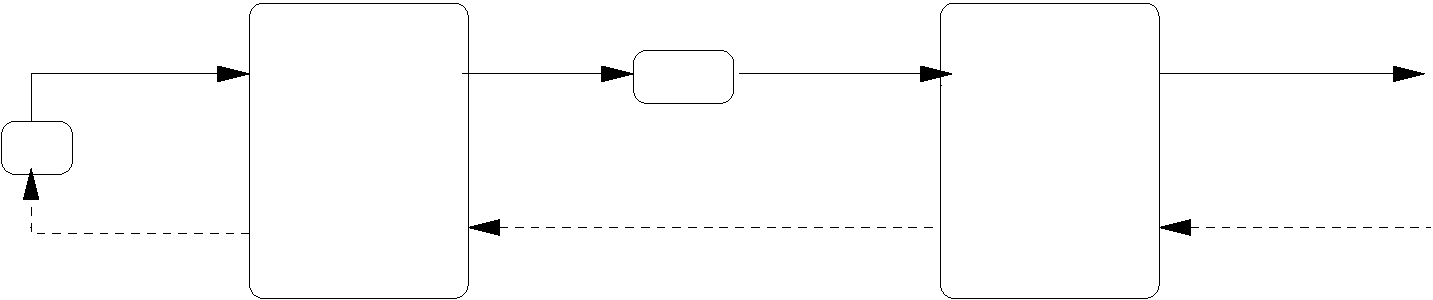
\includegraphics{2node.pdf}%
\end{picture}%
\setlength{\unitlength}{4144sp}%
%
\begingroup\makeatletter\ifx\SetFigFont\undefined%
\gdef\SetFigFont#1#2#3#4#5{%
  \reset@font\fontsize{#1}{#2pt}%
  \fontfamily{#3}\fontseries{#4}\fontshape{#5}%
  \selectfont}%
\fi\endgroup%
\begin{picture}(10914,2274)(1114,-4123)
\put(1936,-3796){\makebox(0,0)[lb]{\smash{{\SetFigFont{12}{14.4}{\familydefault}{\mddefault}{\updefault}{\color[rgb]{0,0,0}$O_{2}(k)$}%
}}}}
\put(11116,-3841){\makebox(0,0)[lb]{\smash{{\SetFigFont{12}{14.4}{\familydefault}{\mddefault}{\updefault}{\color[rgb]{0,0,0}$\Dem(k)$}%
}}}}
\put(1576,-2266){\makebox(0,0)[lb]{\smash{{\SetFigFont{12}{14.4}{\familydefault}{\mddefault}{\updefault}{\color[rgb]{0,0,0}$O_{2}(k-\tau_M)$}%
}}}}
\put(3106,-2986){\makebox(0,0)[lb]{\smash{{\SetFigFont{14}{16.8}{\familydefault}{\mddefault}{\updefault}{\color[rgb]{0,0,0}Manufacturer}%
}}}}
\put(8641,-2986){\makebox(0,0)[lb]{\smash{{\SetFigFont{14}{16.8}{\familydefault}{\mddefault}{\updefault}{\color[rgb]{0,0,0}Retailer}%
}}}}
\put(6166,-2491){\makebox(0,0)[lb]{\smash{{\SetFigFont{10}{12.0}{\familydefault}{\mddefault}{\updefault}{\color[rgb]{0,0,0}$\tau_T=2$}%
}}}}
\put(1171,-3031){\makebox(0,0)[lb]{\smash{{\SetFigFont{10}{12.0}{\familydefault}{\mddefault}{\updefault}{\color[rgb]{0,0,0}$\tau_M = 2$}%
}}}}
\put(8686,-3301){\makebox(0,0)[lb]{\smash{{\SetFigFont{12}{14.4}{\familydefault}{\mddefault}{\updefault}{\color[rgb]{0,0,0}Node $1$}%
}}}}
\put(9991,-2311){\makebox(0,0)[lb]{\smash{{\SetFigFont{12}{14.4}{\familydefault}{\mddefault}{\updefault}{\color[rgb]{0,0,0}$S_{1}(k)$}%
}}}}
\put(7201,-3886){\makebox(0,0)[lb]{\smash{{\SetFigFont{12}{14.4}{\familydefault}{\mddefault}{\updefault}{\color[rgb]{0,0,0}$O_{1}(k)$}%
}}}}
\put(4816,-2716){\makebox(0,0)[lb]{\smash{{\SetFigFont{12}{14.4}{\familydefault}{\mddefault}{\updefault}{\color[rgb]{0,0,0}$S_{2}(k)$}%
}}}}
\put(3421,-3301){\makebox(0,0)[lb]{\smash{{\SetFigFont{12}{14.4}{\familydefault}{\mddefault}{\updefault}{\color[rgb]{0,0,0}Node $2$}%
}}}}
\end{picture}%
}}
\caption{Two-stage supply chain.}
\label{fig:2stage}
\end{figure}

Denoting the state of the supply chain as $x = \begin{bmatrix} \Inv_1
  & \BO_1 & \Inv_2 & \BO_2 \end{bmatrix}'$ and the input as $u
= \begin{bmatrix} S_1 & O_1 & S_2 & O_2 \end{bmatrix}'$, the state
space model for the two-node supply chain can be written as:
\begin{multline}
\label{eq:model0}
\underbrace{\begin{bmatrix}\Inv_1\\\BO_1\\\Inv_2 \\
    \BO_2\end{bmatrix}_{k+1}}_{x(k+1)} = 
\underbrace{\begin{bmatrix} 1 & & &
 \\ & 1 & &\\ & & 1 & \\ & & & 1\end{bmatrix}}_{A}
\underbrace{\begin{bmatrix}\Inv_1\\\BO_1\\\Inv_2 \\
    \BO_2\end{bmatrix}_{k}}_{x(k)}+
\underbrace{\begin{bmatrix}-1&0 &0 &0 \\-1&0 &0 &0 \\
0&0 & -1 &0 \\0 & 1 & -1 &0 \end{bmatrix}}_{B}
\underbrace{\begin{bmatrix}S_{1}\\O_{1}\\S_{2}\\O_{2}\end{bmatrix}_{k}}_{u(k)}+\\
\underbrace{\begin{bmatrix} 0&0 &1 &0 \\0 &0 &0 &0 \\
0&0 &0  &1 \\0 & 0 &0  &0 \end{bmatrix}}_{B^{(2)}}
\underbrace{\begin{bmatrix}S_{1}\\O_{1}\\S_{2}\\O_{2}\end{bmatrix}_{k-2}}_{u(k-2)}+
\underbrace{\begin{bmatrix}0 \\ 1 \\0 \\0 \end{bmatrix}}_{B_d}\underbrace{\begin{bmatrix}\Dem\end{bmatrix}_{k}}_{d(k)}
\end{multline}

The equation \eqref{eq:model0} can be easily written in the form
\eqref{eq:model} by redefining the state $x(k)
\leftarrow \begin{bmatrix}x(k) & u(k-1) & u(k-2) \end{bmatrix}'$.
We use the following economic stage cost denoted by $\ell_E$ (to
distinguish from the tracking stage cost $\ell_T$ that is introduced
subsequently) as:
\[ \ell_E(x,u)  = q'x + r'u\]
The vector $q$ consists of the inventory holding cost and lost sales
penalty, while the vector $r$ consists of shipping and ordering/production
costs.   
The input constraints consist of the non-negativity of the shipments
and orders and the maximum production/shipping between nodes. It is
represented as: 
\[ {0} = \begin{bmatrix}0\\0\\0\\0\end{bmatrix} \leq Iu \leq
  \begin{bmatrix} \bar{S_1} \\ \bar{O_1} \\ \bar{S_2}
    \\ \bar{O_2} \end{bmatrix} = \bar{u} \]
in which $I$ is the identity matrix.
Similarly, the state constraint consists of the non-negativity
constraints and the maximum inventory capacity. It is represented as:
\[ {0} = \begin{bmatrix}0\\0\\0\\0\end{bmatrix} \leq Ix \leq
  \begin{bmatrix} \bar{\Inv_1} \\ \bar{\BO_1} \\ \bar{\Inv_2}
    \\ \bar{\BO_2} \end{bmatrix} = \bar{x} \]
With this model definition and constraint sets, the steady-state
optimization problem \eqref{eq:SS} decomposes into two separate
problems (because the state matrix in \eqref{eq:model0} is the
identity matrix) as:
\begin{equation}
\label{eq:esc:SSx} \min_{x}{q'x} \qquad \text{s.t.~} {0} \leq Ix
\leq \bar{x}
\end{equation}
and
\begin{equation}
\label{eq:esc:SSu} \min_{u}{r'u} \qquad \text{s.t.~}  B^{(2)}u +
Bu + B_dd_s = 0,
 {0} \leq Iu\leq \bar{u}
\end{equation}
For non-negative costs in the vector $q$, the solution to the linear
program \eqref{eq:esc:SSx} is ${0}$, i.e., the economically
optimal operating point is to hold no inventories and
backorders. Corresponding to this steady state $x_s = {0}$,
the economic shipping quantities (in response to nominal demands) is
such that $B^{(2)}u_s + Bu_s = -B_dd_s$, i.e., all the flows in the supply
  chain are balanced (and for this 2 node example, it means that all
  the flows are equal to the customer demand). The economic cost of
  operating at the steady state is $r'u_s$.

\subsection{Results}
\label{sec:ecoMPC_res}
First, we show that simple rolling horizon optimization without
terminal constraints can lead to unfavorable closed-loop solutions. We
choose the stage cost $\ell(x,u) = q'x + r'u$ in which the costs $q,r$
are chosen as follows:
\[ q = (1,1,1,0.01)' \qquad r = (10,0.1,10,1)' \]
Note that the shipping cost is 10, and it is much greater than the
backorder cost (1,0.01).  In this
simulation study,the
maximum production/shipping between the nodes is 20 units every time
period.

The optimization problem solved is one
without terminal constraint and is given by
\eqref{eq:PN_none}
\begin{xalignat}{2}
\label{eq:PN_none}
\mathbb{P}_N(x;d_s) :& \min_{\bu}{V_N(\bu;x)} & \nonumber \\
&\text{s.t.~} x(j+1) = Ax(j) + Bu(j) +B_dd_s, & j \in
\mathbb{I}_{0:N-1} \nonumber \\
&x(j) \in \mathbb{X}& j \in \mathbb{I}_{0:N-1} \\
&u(j) \in \mathbb{U}& j \in \mathbb{I}_{0:N-1} \nonumber 
%&x(N) = \mathbb{X}_f & \nonumber
\end{xalignat}
in which $V_N(\bu;x)$ is given by \eqref{eq:VN_equality}. The stage cost used is $\ell_E(x,u)$.
In Figure \ref{fig:esc:unstable_SC}, we show the closed-loop response to the
rolling horizon implementation in which \eqref{eq:PN_none} is solved
online at each sampling time. The prediction horizon $N$ is 15. The
system started at the economic steady state $(x_s,u_s;d_s)$. We observe
that despite implementing the optimal input at each sampling time, the
backorder increases with time, indicating that the demands are not
being met (for this choice of costs and control horizon). Hence, the
closed-loop economic cost is increasing with time, while
there exists a cheaper solution of staying on the steady state and
bearing a cost of $r'u_s$ at each time. 

In Figure \ref{fig:esc:stable_SC}, we show the closed-loop response to
the MPC implementation in which optimization problem
\eqref{eq:PN_equality} is solved at each sampling instance. We start
from an initial condition that is not the steady state. Notice that
the closed-loop response quickly settles to the optimal economic steady
state. Hence, by using economic MPC theory, we could stabilize a
supply chain, even with a pathological cost vector. 

\begin{figure}
\centering
\small
{\resizebox{\textwidth}{!}{% GNUPLOT: LaTeX picture with Postscript
\begingroup
  \makeatletter
  \providecommand\color[2][]{%
    \GenericError{(gnuplot) \space\space\space\@spaces}{%
      Package color not loaded in conjunction with
      terminal option `colourtext'%
    }{See the gnuplot documentation for explanation.%
    }{Either use 'blacktext' in gnuplot or load the package
      color.sty in LaTeX.}%
    \renewcommand\color[2][]{}%
  }%
  \providecommand\includegraphics[2][]{%
    \GenericError{(gnuplot) \space\space\space\@spaces}{%
      Package graphicx or graphics not loaded%
    }{See the gnuplot documentation for explanation.%
    }{The gnuplot epslatex terminal needs graphicx.sty or graphics.sty.}%
    \renewcommand\includegraphics[2][]{}%
  }%
  \providecommand\rotatebox[2]{#2}%
  \@ifundefined{ifGPcolor}{%
    \newif\ifGPcolor
    \GPcolorfalse
  }{}%
  \@ifundefined{ifGPblacktext}{%
    \newif\ifGPblacktext
    \GPblacktexttrue
  }{}%
  % define a \g@addto@macro without @ in the name:
  \let\gplgaddtomacro\g@addto@macro
  % define empty templates for all commands taking text:
  \gdef\gplbacktext{}%
  \gdef\gplfronttext{}%
  \makeatother
  \ifGPblacktext
    % no textcolor at all
    \def\colorrgb#1{}%
    \def\colorgray#1{}%
  \else
    % gray or color?
    \ifGPcolor
      \def\colorrgb#1{\color[rgb]{#1}}%
      \def\colorgray#1{\color[gray]{#1}}%
      \expandafter\def\csname LTw\endcsname{\color{white}}%
      \expandafter\def\csname LTb\endcsname{\color{black}}%
      \expandafter\def\csname LTa\endcsname{\color{black}}%
      \expandafter\def\csname LT0\endcsname{\color[rgb]{1,0,0}}%
      \expandafter\def\csname LT1\endcsname{\color[rgb]{0,1,0}}%
      \expandafter\def\csname LT2\endcsname{\color[rgb]{0,0,1}}%
      \expandafter\def\csname LT3\endcsname{\color[rgb]{1,0,1}}%
      \expandafter\def\csname LT4\endcsname{\color[rgb]{0,1,1}}%
      \expandafter\def\csname LT5\endcsname{\color[rgb]{1,1,0}}%
      \expandafter\def\csname LT6\endcsname{\color[rgb]{0,0,0}}%
      \expandafter\def\csname LT7\endcsname{\color[rgb]{1,0.3,0}}%
      \expandafter\def\csname LT8\endcsname{\color[rgb]{0.5,0.5,0.5}}%
    \else
      % gray
      \def\colorrgb#1{\color{black}}%
      \def\colorgray#1{\color[gray]{#1}}%
      \expandafter\def\csname LTw\endcsname{\color{white}}%
      \expandafter\def\csname LTb\endcsname{\color{black}}%
      \expandafter\def\csname LTa\endcsname{\color{black}}%
      \expandafter\def\csname LT0\endcsname{\color{black}}%
      \expandafter\def\csname LT1\endcsname{\color{black}}%
      \expandafter\def\csname LT2\endcsname{\color{black}}%
      \expandafter\def\csname LT3\endcsname{\color{black}}%
      \expandafter\def\csname LT4\endcsname{\color{black}}%
      \expandafter\def\csname LT5\endcsname{\color{black}}%
      \expandafter\def\csname LT6\endcsname{\color{black}}%
      \expandafter\def\csname LT7\endcsname{\color{black}}%
      \expandafter\def\csname LT8\endcsname{\color{black}}%
    \fi
  \fi
  \setlength{\unitlength}{0.0500bp}%
  \begin{picture}(7200.00,3024.00)%
    \gplgaddtomacro\gplbacktext{%
      \csname LTb\endcsname%
      \put(1078,714){\makebox(0,0)[r]{\strut{} 0}}%
      \put(1078,1225){\makebox(0,0)[r]{\strut{} 500}}%
      \put(1078,1737){\makebox(0,0)[r]{\strut{} 1000}}%
      \put(1078,2248){\makebox(0,0)[r]{\strut{} 1500}}%
      \put(1078,2759){\makebox(0,0)[r]{\strut{} 2000}}%
      \put(1210,484){\makebox(0,0){\strut{} 0}}%
      \put(2329,484){\makebox(0,0){\strut{} 40}}%
      \put(3447,484){\makebox(0,0){\strut{} 80}}%
      \put(4566,484){\makebox(0,0){\strut{} 120}}%
      \put(5684,484){\makebox(0,0){\strut{} 160}}%
      \put(6803,484){\makebox(0,0){\strut{} 200}}%
      \put(176,1731){\rotatebox{-270}{\makebox(0,0){\strut{}Backorder -Retailer}}}%
      \put(4006,154){\makebox(0,0){\strut{}Time}}%
    }%
    \gplgaddtomacro\gplfronttext{%
    }%
    \gplbacktext
    \put(0,0){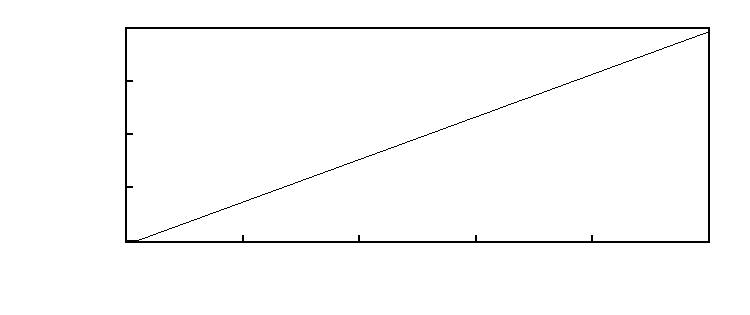
\includegraphics{unstable_SC.pdf}}%
    \gplfronttext
  \end{picture}%
\endgroup
}}
\caption{Backorder in the retailer for rolling horizon optimization
  without stability constraints.}
\label{fig:esc:unstable_SC}
\end{figure}

\begin{figure}
\centering
\scriptsize
{\resizebox{\textwidth}{!}{% GNUPLOT: LaTeX picture with Postscript
\begingroup
  \makeatletter
  \providecommand\color[2][]{%
    \GenericError{(gnuplot) \space\space\space\@spaces}{%
      Package color not loaded in conjunction with
      terminal option `colourtext'%
    }{See the gnuplot documentation for explanation.%
    }{Either use 'blacktext' in gnuplot or load the package
      color.sty in LaTeX.}%
    \renewcommand\color[2][]{}%
  }%
  \providecommand\includegraphics[2][]{%
    \GenericError{(gnuplot) \space\space\space\@spaces}{%
      Package graphicx or graphics not loaded%
    }{See the gnuplot documentation for explanation.%
    }{The gnuplot epslatex terminal needs graphicx.sty or graphics.sty.}%
    \renewcommand\includegraphics[2][]{}%
  }%
  \providecommand\rotatebox[2]{#2}%
  \@ifundefined{ifGPcolor}{%
    \newif\ifGPcolor
    \GPcolorfalse
  }{}%
  \@ifundefined{ifGPblacktext}{%
    \newif\ifGPblacktext
    \GPblacktexttrue
  }{}%
  % define a \g@addto@macro without @ in the name:
  \let\gplgaddtomacro\g@addto@macro
  % define empty templates for all commands taking text:
  \gdef\gplbacktext{}%
  \gdef\gplfronttext{}%
  \makeatother
  \ifGPblacktext
    % no textcolor at all
    \def\colorrgb#1{}%
    \def\colorgray#1{}%
  \else
    % gray or color?
    \ifGPcolor
      \def\colorrgb#1{\color[rgb]{#1}}%
      \def\colorgray#1{\color[gray]{#1}}%
      \expandafter\def\csname LTw\endcsname{\color{white}}%
      \expandafter\def\csname LTb\endcsname{\color{black}}%
      \expandafter\def\csname LTa\endcsname{\color{black}}%
      \expandafter\def\csname LT0\endcsname{\color[rgb]{1,0,0}}%
      \expandafter\def\csname LT1\endcsname{\color[rgb]{0,1,0}}%
      \expandafter\def\csname LT2\endcsname{\color[rgb]{0,0,1}}%
      \expandafter\def\csname LT3\endcsname{\color[rgb]{1,0,1}}%
      \expandafter\def\csname LT4\endcsname{\color[rgb]{0,1,1}}%
      \expandafter\def\csname LT5\endcsname{\color[rgb]{1,1,0}}%
      \expandafter\def\csname LT6\endcsname{\color[rgb]{0,0,0}}%
      \expandafter\def\csname LT7\endcsname{\color[rgb]{1,0.3,0}}%
      \expandafter\def\csname LT8\endcsname{\color[rgb]{0.5,0.5,0.5}}%
    \else
      % gray
      \def\colorrgb#1{\color{black}}%
      \def\colorgray#1{\color[gray]{#1}}%
      \expandafter\def\csname LTw\endcsname{\color{white}}%
      \expandafter\def\csname LTb\endcsname{\color{black}}%
      \expandafter\def\csname LTa\endcsname{\color{black}}%
      \expandafter\def\csname LT0\endcsname{\color{black}}%
      \expandafter\def\csname LT1\endcsname{\color{black}}%
      \expandafter\def\csname LT2\endcsname{\color{black}}%
      \expandafter\def\csname LT3\endcsname{\color{black}}%
      \expandafter\def\csname LT4\endcsname{\color{black}}%
      \expandafter\def\csname LT5\endcsname{\color{black}}%
      \expandafter\def\csname LT6\endcsname{\color{black}}%
      \expandafter\def\csname LT7\endcsname{\color{black}}%
      \expandafter\def\csname LT8\endcsname{\color{black}}%
    \fi
  \fi
  \setlength{\unitlength}{0.0500bp}%
  \begin{picture}(7200.00,3024.00)%
    \gplgaddtomacro\gplbacktext{%
      \csname LTb\endcsname%
      \put(814,832){\makebox(0,0)[r]{\strut{} 0}}%
      \put(814,1475){\makebox(0,0)[r]{\strut{} 10}}%
      \put(814,2117){\makebox(0,0)[r]{\strut{} 20}}%
      \put(814,2759){\makebox(0,0)[r]{\strut{} 30}}%
      \put(946,484){\makebox(0,0){\strut{} 0}}%
      \put(1433,484){\makebox(0,0){\strut{} 2}}%
      \put(1921,484){\makebox(0,0){\strut{} 4}}%
      \put(2408,484){\makebox(0,0){\strut{} 6}}%
      \put(2896,484){\makebox(0,0){\strut{} 8}}%
      \put(3383,484){\makebox(0,0){\strut{} 10}}%
      \put(176,1731){\rotatebox{-270}{\makebox(0,0){\strut{}Inventory}}}%
      \put(2164,154){\makebox(0,0){\strut{}Time}}%
    }%
    \gplgaddtomacro\gplfronttext{%
      \csname LTb\endcsname%
      \put(2061,2970){\makebox(0,0)[r]{\strut{}Retailer}}%
    }%
    \gplgaddtomacro\gplbacktext{%
      \csname LTb\endcsname%
      \put(4109,484){\makebox(0,0){\strut{} 0}}%
      \put(4544,484){\makebox(0,0){\strut{} 2}}%
      \put(4978,484){\makebox(0,0){\strut{} 4}}%
      \put(5413,484){\makebox(0,0){\strut{} 6}}%
      \put(5847,484){\makebox(0,0){\strut{} 8}}%
      \put(6282,484){\makebox(0,0){\strut{} 10}}%
      \put(6414,998){\makebox(0,0)[l]{\strut{} 0}}%
      \put(6414,2465){\makebox(0,0)[l]{\strut{} 10}}%
      \put(7051,1731){\rotatebox{-270}{\makebox(0,0){\strut{}Backorder}}}%
      \put(5195,154){\makebox(0,0){\strut{}Time}}%
    }%
    \gplgaddtomacro\gplfronttext{%
      \csname LTb\endcsname%
      \put(5039,2943){\makebox(0,0)[r]{\strut{}Manufacturer}}%
    }%
    \gplbacktext
    \put(0,0){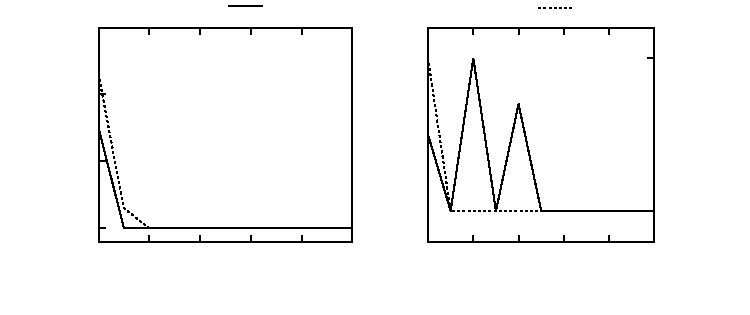
\includegraphics{stable_SC.pdf}}%
    \gplfronttext
  \end{picture}%
\endgroup
}}
\caption{Closed loop evolution using stabilizing MPC.}
\label{fig:esc:stable_SC}
\end{figure}

For this simple two-node supply chain, we show that simple
reoptimization can lead to unfavorable solutions. Although, we use an
unfavorable cost function, for larger, complex networks, it can be
hard to a priori judge if simple reoptimizations can lead to favorable
solutions. On the other hand, using economic MPC theory, we have
guarantees on the closed-loop performance. 

\subsection{Multiobjective stage cost}
\label{sec:multiobj}
Supply chain managers wish to balance profit maximization with 
risk minimization. One way to minimize risk is to hold some buffer
stock so that the supply chain can respond to rush orders or demand
spikes. As seen in the previous section, the unique economic steady
state (for a non-negative cost vector $q$) is ${0}$. That
is, the economic optimum is to carry no stock. In this section, we
introduce a multiobjective stage cost, which is a weighted sum of the
economic stage cost discussed in the previous section and a tracking
stage cost. The multiobjective stage cost is of the form:
\begin{equation}
\label{eq:esc:ell}
\ell(x,u) = \frac{\omega}{s_E} \ell_E(x,u) + \frac{(1-\omega)}{s_T} \ell_T(x,u;z_t)
\end{equation}
in which the parameter $\omega \in [0,1]$ is a relative weighting
given to the economic costs and the tracking cost. The function
$\ell_T(x,u;z_t)$ is the tracking stage cost, which penalizes the
deviations from a safety stock (chosen to be a steady state of
\eqref{eq:model0}) $z_t = (x_t,u_t)$. The tracking stage cost
is defined as:
\begin{equation}
\label{eq:esc:ellT}
\ell_T(x,u;z_t) = 1/2(x-x_t)'Q(x-x_t)+ 1/2(u-u_t)'R(u-u_t)
\end{equation} 

The parameters $s_T,s_E$ are scaling parameters. To obtain the scaling
parameters, we consider the utopia and nadir points of the individual
stage costs $\ell_E(x,u)$ and $\ell_T(x,u)$
\cite{kim:weck:2005}. Denote $z=(x,u)$. We solve
\[ z_E = \text{arg}\min_{z \in \mathbb{X} \times \mathbb{U}}{\ell_E(x,u)}, \quad z_T = \text{arg}\min_{z \in \mathbb{X} \times
  \mathbb{U}}{\ell_T(x,u;z_t)} \]
The utopia point is the best possible costs that can be attained for
both the cost functions:
\[J^U = (\ell_E(z_E),\ell_T(z_T;z_t))\in
\mathbb{R}^2\] 
The nadir point is the cost attained by one stage cost at the optimal
solution of the other stage cost.
\[J^N = (\ell_E(z_T),\ell_T(z_E;z_t))\in
\mathbb{R}^2 \] 
The parameters $s_T,s_E$ are then defined as:
\[ (s_E,s_T) = J^N-J^U \]
Also, we chose $u_t = u_s$, the economic steady state, because as
mentioned earlier, the steady-state inputs are independent of the
steady-state inventories and only depend on the nominal demand.
The steady-state problem now can be written as:
\begin{align}
\label{eq:esc:SSMulti}
&\min_{x,u}{}(\frac{\omega}{s_E} (q'x+r'u) +
\frac{(1-\omega)}{s_T}((x-x_t)'Q(x-x_{t})+(u-u_s)'R(u-u_s)))
\nonumber\\
&\text{s.t.~} x=Ax+Bu+B_dd_s, u \in \mathbb{U}, x \in \mathbb{X} 
\end{align}

Note that the steady state obtained is a function of the parameter $\omega$.
When $\omega = 0$, the steady state is $(x_t,u_s)$. On the other hand,
when $\omega = 1$, the steady state is $({0},u_s)$. Hence,
the parameter $\omega$ captures the manager's relative importance
of profit and risk. For $\omega = 0$, 
the manager is risk averse, while $\omega = 1$ implies that the
manager is risk seeking. In Figure \ref{fig:esc:SS_omega}, we plot
the inventory steady state as a function of $\omega$. We chose the
backorder targets $\BO_{1,t} = \BO_{2,t} = 0$. Therefore, irrespective
of $\omega$, the backorder steady state is $0$. The parameters used
are  $ Q =
10\diag{(1,1,1,1)}, R = 10^{-5}\diag{(1,1,1,1)}$, $x_{t}
= (35,0,45,0)$. The economic costs are $q = (10,10,10,1), r =
(10,0.1,10,100)$. The nominal demand is $d_s = 10$. 

\begin{figure}
\centering
\scriptsize
{\resizebox{\textwidth}{!}{% GNUPLOT: LaTeX picture with Postscript
\begingroup
  \makeatletter
  \providecommand\color[2][]{%
    \GenericError{(gnuplot) \space\space\space\@spaces}{%
      Package color not loaded in conjunction with
      terminal option `colourtext'%
    }{See the gnuplot documentation for explanation.%
    }{Either use 'blacktext' in gnuplot or load the package
      color.sty in LaTeX.}%
    \renewcommand\color[2][]{}%
  }%
  \providecommand\includegraphics[2][]{%
    \GenericError{(gnuplot) \space\space\space\@spaces}{%
      Package graphicx or graphics not loaded%
    }{See the gnuplot documentation for explanation.%
    }{The gnuplot epslatex terminal needs graphicx.sty or graphics.sty.}%
    \renewcommand\includegraphics[2][]{}%
  }%
  \providecommand\rotatebox[2]{#2}%
  \@ifundefined{ifGPcolor}{%
    \newif\ifGPcolor
    \GPcolorfalse
  }{}%
  \@ifundefined{ifGPblacktext}{%
    \newif\ifGPblacktext
    \GPblacktexttrue
  }{}%
  % define a \g@addto@macro without @ in the name:
  \let\gplgaddtomacro\g@addto@macro
  % define empty templates for all commands taking text:
  \gdef\gplbacktext{}%
  \gdef\gplfronttext{}%
  \makeatother
  \ifGPblacktext
    % no textcolor at all
    \def\colorrgb#1{}%
    \def\colorgray#1{}%
  \else
    % gray or color?
    \ifGPcolor
      \def\colorrgb#1{\color[rgb]{#1}}%
      \def\colorgray#1{\color[gray]{#1}}%
      \expandafter\def\csname LTw\endcsname{\color{white}}%
      \expandafter\def\csname LTb\endcsname{\color{black}}%
      \expandafter\def\csname LTa\endcsname{\color{black}}%
      \expandafter\def\csname LT0\endcsname{\color[rgb]{1,0,0}}%
      \expandafter\def\csname LT1\endcsname{\color[rgb]{0,1,0}}%
      \expandafter\def\csname LT2\endcsname{\color[rgb]{0,0,1}}%
      \expandafter\def\csname LT3\endcsname{\color[rgb]{1,0,1}}%
      \expandafter\def\csname LT4\endcsname{\color[rgb]{0,1,1}}%
      \expandafter\def\csname LT5\endcsname{\color[rgb]{1,1,0}}%
      \expandafter\def\csname LT6\endcsname{\color[rgb]{0,0,0}}%
      \expandafter\def\csname LT7\endcsname{\color[rgb]{1,0.3,0}}%
      \expandafter\def\csname LT8\endcsname{\color[rgb]{0.5,0.5,0.5}}%
    \else
      % gray
      \def\colorrgb#1{\color{black}}%
      \def\colorgray#1{\color[gray]{#1}}%
      \expandafter\def\csname LTw\endcsname{\color{white}}%
      \expandafter\def\csname LTb\endcsname{\color{black}}%
      \expandafter\def\csname LTa\endcsname{\color{black}}%
      \expandafter\def\csname LT0\endcsname{\color{black}}%
      \expandafter\def\csname LT1\endcsname{\color{black}}%
      \expandafter\def\csname LT2\endcsname{\color{black}}%
      \expandafter\def\csname LT3\endcsname{\color{black}}%
      \expandafter\def\csname LT4\endcsname{\color{black}}%
      \expandafter\def\csname LT5\endcsname{\color{black}}%
      \expandafter\def\csname LT6\endcsname{\color{black}}%
      \expandafter\def\csname LT7\endcsname{\color{black}}%
      \expandafter\def\csname LT8\endcsname{\color{black}}%
    \fi
  \fi
  \setlength{\unitlength}{0.0500bp}%
  \begin{picture}(7200.00,3024.00)%
    \gplgaddtomacro\gplbacktext{%
      \csname LTb\endcsname%
      \put(814,802){\makebox(0,0)[r]{\strut{} 0}}%
      \put(814,1291){\makebox(0,0)[r]{\strut{} 10}}%
      \put(814,1780){\makebox(0,0)[r]{\strut{} 20}}%
      \put(814,2270){\makebox(0,0)[r]{\strut{} 30}}%
      \put(814,2759){\makebox(0,0)[r]{\strut{} 40}}%
      \put(946,484){\makebox(0,0){\strut{} 0}}%
      \put(1433,484){\makebox(0,0){\strut{} 0.2}}%
      \put(1921,484){\makebox(0,0){\strut{} 0.4}}%
      \put(2408,484){\makebox(0,0){\strut{} 0.6}}%
      \put(2896,484){\makebox(0,0){\strut{} 0.8}}%
      \put(3383,484){\makebox(0,0){\strut{} 1}}%
      \put(176,1731){\rotatebox{-270}{\makebox(0,0){\strut{}Inventory}}}%
      \put(2164,154){\makebox(0,0){\strut{}$\omega$}}%
      \put(2165,2514){\makebox(0,0){\strut{}Retailer}}%
    }%
    \gplgaddtomacro\gplfronttext{%
    }%
    \gplgaddtomacro\gplbacktext{%
      \csname LTb\endcsname%
      \put(4109,484){\makebox(0,0){\strut{} 0}}%
      \put(4544,484){\makebox(0,0){\strut{} 0.2}}%
      \put(4978,484){\makebox(0,0){\strut{} 0.4}}%
      \put(5413,484){\makebox(0,0){\strut{} 0.6}}%
      \put(5847,484){\makebox(0,0){\strut{} 0.8}}%
      \put(6282,484){\makebox(0,0){\strut{} 1}}%
      \put(6414,791){\makebox(0,0)[l]{\strut{} 0}}%
      \put(6414,1229){\makebox(0,0)[l]{\strut{} 10}}%
      \put(6414,1666){\makebox(0,0)[l]{\strut{} 20}}%
      \put(6414,2103){\makebox(0,0)[l]{\strut{} 30}}%
      \put(6414,2540){\makebox(0,0)[l]{\strut{} 40}}%
      \put(7051,1731){\rotatebox{-270}{\makebox(0,0){\strut{}Inventory}}}%
      \put(5195,154){\makebox(0,0){\strut{}$\omega$}}%
      \put(5196,2514){\makebox(0,0){\strut{}Manufacturer}}%
    }%
    \gplgaddtomacro\gplfronttext{%
    }%
    \gplbacktext
    \put(0,0){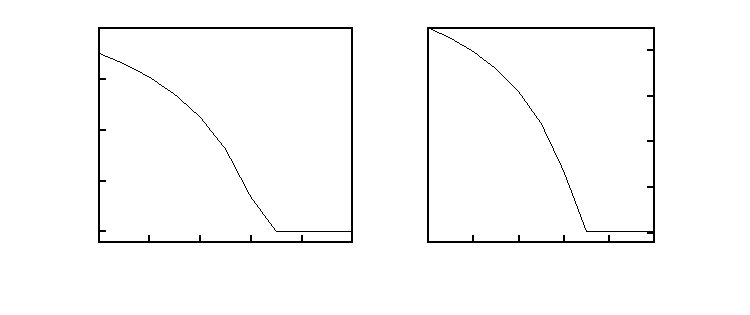
\includegraphics{SS_omega.pdf}}%
    \gplfronttext
  \end{picture}%
\endgroup
}}
\caption{Steady state as a function of the relative weighting between
  tracking and  economics}
\label{fig:esc:SS_omega}
\end{figure}

In this section we use the terminal
penalty formulation, \eqref{eq:PN_region} as the centralized MPC optimization problem.  We can also formulate the on-line MPC problem using optimization
problem \eqref{eq:PN_equality},

To obtain the terminal region and penalty, we first have to find the
terminal controller $\kappa_f(x)$. For the supply chain model, we
choose the controller $\kappa_f(x) = Kx$. Since the optimal steady
state for a fixed value of $\omega$ implies that the backorders at
both the nodes are zero, i.e., some state constraints are active at the steady state, we use the method outlined in
\cite{rao:rawlings:1999} to obtain the feedback gain. It is important
to note that when the steady-state inventories are also zero (for
example, when $\omega = 1$), then we can use only the terminal
constraint problem \eqref{eq:PN_equality}, because the theory
in \cite{rao:rawlings:1999} reduces to an equality constraint for this
case. Given the choice of
feedback gain $K$, we have that $A_K := A+BK$ is stable (i.e., all
eigenvalues of $A_K$ are strictly inside the unit circle). Defining
$Q_K = Q+K'RK$ and $q_k = q+K'r$, we can choose the terminal penalty
to be:
\begin{equation}
\label{eq:esc:Vf}
V_f(x;x_s) = (x-x_s)'P(x-x_s)+ p'(x-x_s)
\end{equation}
in which the positive definite matrix $P$ is the solution to the
Lyapunov equation
\[ A_K'PA_K-P = -Q_K \]
and $p$ is the solution to 
\[ (A_K-I)'p = -q_K \]
In order to satisfy the basic stability assumption, we require
that  
\begin{equation}
\label{eq:esc:BSA_condition}
(x-x_s)'Q(x_s-x_t)  \leq 0
\end{equation}
Having found $\kappa_f(x) = Kx, V_f(x) = 1/2x'Px + p'x$, the terminal
region can be found by using condition \eqref{eq:esc:BSA_condition}
along with algorithms to find the maximal output admissible set (see
\cite{gilbert:tan:1991, kvasnica:grieder:baotic:2006} for algorithms).

In Figure \ref{fig:esc:CL}, we plot the closed-loop response for three
different values of $\omega$. The online MPC problem solved is \eqref{eq:PN_region} with objective function given by \eqref{eq:VN_region}. The stage cost is given by \eqref{eq:esc:ell} while the terminal function is chosen using the above mentioned method.  Alongside, we also plot the response for
pure-tracking ($\omega = 0$) to the same steady state. That is,  we use the stage cost as $\ell_T(x,u;z_s)$ in which $z_s = (x_s,u_s)$ is the steady state of the multiobjective formulation. 

\begin{figure*}
\centering
\scriptsize
{\resizebox{\textwidth}{!}{% GNUPLOT: LaTeX picture with Postscript
\begingroup
  \makeatletter
  \providecommand\color[2][]{%
    \GenericError{(gnuplot) \space\space\space\@spaces}{%
      Package color not loaded in conjunction with
      terminal option `colourtext'%
    }{See the gnuplot documentation for explanation.%
    }{Either use 'blacktext' in gnuplot or load the package
      color.sty in LaTeX.}%
    \renewcommand\color[2][]{}%
  }%
  \providecommand\includegraphics[2][]{%
    \GenericError{(gnuplot) \space\space\space\@spaces}{%
      Package graphicx or graphics not loaded%
    }{See the gnuplot documentation for explanation.%
    }{The gnuplot epslatex terminal needs graphicx.sty or graphics.sty.}%
    \renewcommand\includegraphics[2][]{}%
  }%
  \providecommand\rotatebox[2]{#2}%
  \@ifundefined{ifGPcolor}{%
    \newif\ifGPcolor
    \GPcolorfalse
  }{}%
  \@ifundefined{ifGPblacktext}{%
    \newif\ifGPblacktext
    \GPblacktexttrue
  }{}%
  % define a \g@addto@macro without @ in the name:
  \let\gplgaddtomacro\g@addto@macro
  % define empty templates for all commands taking text:
  \gdef\gplbacktext{}%
  \gdef\gplfronttext{}%
  \makeatother
  \ifGPblacktext
    % no textcolor at all
    \def\colorrgb#1{}%
    \def\colorgray#1{}%
  \else
    % gray or color?
    \ifGPcolor
      \def\colorrgb#1{\color[rgb]{#1}}%
      \def\colorgray#1{\color[gray]{#1}}%
      \expandafter\def\csname LTw\endcsname{\color{white}}%
      \expandafter\def\csname LTb\endcsname{\color{black}}%
      \expandafter\def\csname LTa\endcsname{\color{black}}%
      \expandafter\def\csname LT0\endcsname{\color[rgb]{1,0,0}}%
      \expandafter\def\csname LT1\endcsname{\color[rgb]{0,1,0}}%
      \expandafter\def\csname LT2\endcsname{\color[rgb]{0,0,1}}%
      \expandafter\def\csname LT3\endcsname{\color[rgb]{1,0,1}}%
      \expandafter\def\csname LT4\endcsname{\color[rgb]{0,1,1}}%
      \expandafter\def\csname LT5\endcsname{\color[rgb]{1,1,0}}%
      \expandafter\def\csname LT6\endcsname{\color[rgb]{0,0,0}}%
      \expandafter\def\csname LT7\endcsname{\color[rgb]{1,0.3,0}}%
      \expandafter\def\csname LT8\endcsname{\color[rgb]{0.5,0.5,0.5}}%
    \else
      % gray
      \def\colorrgb#1{\color{black}}%
      \def\colorgray#1{\color[gray]{#1}}%
      \expandafter\def\csname LTw\endcsname{\color{white}}%
      \expandafter\def\csname LTb\endcsname{\color{black}}%
      \expandafter\def\csname LTa\endcsname{\color{black}}%
      \expandafter\def\csname LT0\endcsname{\color{black}}%
      \expandafter\def\csname LT1\endcsname{\color{black}}%
      \expandafter\def\csname LT2\endcsname{\color{black}}%
      \expandafter\def\csname LT3\endcsname{\color{black}}%
      \expandafter\def\csname LT4\endcsname{\color{black}}%
      \expandafter\def\csname LT5\endcsname{\color{black}}%
      \expandafter\def\csname LT6\endcsname{\color{black}}%
      \expandafter\def\csname LT7\endcsname{\color{black}}%
      \expandafter\def\csname LT8\endcsname{\color{black}}%
    \fi
  \fi
  \setlength{\unitlength}{0.0500bp}%
  \begin{picture}(7200.00,3024.00)%
    \gplgaddtomacro\gplbacktext{%
      \csname LTb\endcsname%
      \put(814,704){\makebox(0,0)[r]{\strut{} 10}}%
      \put(814,1257){\makebox(0,0)[r]{\strut{} 20}}%
      \put(814,1810){\makebox(0,0)[r]{\strut{} 30}}%
      \put(814,2363){\makebox(0,0)[r]{\strut{} 40}}%
      \put(946,484){\makebox(0,0){\strut{} 0}}%
      \put(1190,484){\makebox(0,0){\strut{} 2}}%
      \put(1433,484){\makebox(0,0){\strut{} 4}}%
      \put(1677,484){\makebox(0,0){\strut{} 6}}%
      \put(1921,484){\makebox(0,0){\strut{} 8}}%
      \put(2165,484){\makebox(0,0){\strut{} 10}}%
      \put(2408,484){\makebox(0,0){\strut{} 12}}%
      \put(2652,484){\makebox(0,0){\strut{} 14}}%
      \put(2896,484){\makebox(0,0){\strut{} 16}}%
      \put(3139,484){\makebox(0,0){\strut{} 18}}%
      \put(3383,484){\makebox(0,0){\strut{} 20}}%
      \put(176,1533){\rotatebox{-270}{\makebox(0,0){\strut{}Inventory}}}%
      \put(2164,154){\makebox(0,0){\strut{}Time}}%
      \put(2164,2693){\makebox(0,0){\strut{}Retailer}}%
      \put(1921,2087){\makebox(0,0)[l]{\strut{}$\omega = 0.2$}}%
    }%
    \gplgaddtomacro\gplfronttext{%
      \csname LTb\endcsname%
      \put(2548,1147){\makebox(0,0)[r]{\strut{}$\ell(x,u,z_p)$}}%
    }%
    \gplgaddtomacro\gplbacktext{%
      \csname LTb\endcsname%
      \put(4109,484){\makebox(0,0){\strut{} 0}}%
      \put(4326,484){\makebox(0,0){\strut{} 2}}%
      \put(4544,484){\makebox(0,0){\strut{} 4}}%
      \put(4761,484){\makebox(0,0){\strut{} 6}}%
      \put(4978,484){\makebox(0,0){\strut{} 8}}%
      \put(5196,484){\makebox(0,0){\strut{} 10}}%
      \put(5413,484){\makebox(0,0){\strut{} 12}}%
      \put(5630,484){\makebox(0,0){\strut{} 14}}%
      \put(5847,484){\makebox(0,0){\strut{} 16}}%
      \put(6065,484){\makebox(0,0){\strut{} 18}}%
      \put(6282,484){\makebox(0,0){\strut{} 20}}%
      \put(6414,704){\makebox(0,0)[l]{\strut{} 20}}%
      \put(6414,1534){\makebox(0,0)[l]{\strut{} 30}}%
      \put(6414,2363){\makebox(0,0)[l]{\strut{} 40}}%
      \put(7051,1533){\rotatebox{-270}{\makebox(0,0){\strut{}Inventory}}}%
      \put(5195,154){\makebox(0,0){\strut{}Time}}%
      \put(5195,2693){\makebox(0,0){\strut{}Manufacturer}}%
    }%
    \gplgaddtomacro\gplfronttext{%
      \csname LTb\endcsname%
      \put(5474,1175){\makebox(0,0)[r]{\strut{}$\ell_T(x,u,z_s)$}}%
    }%
    \gplbacktext
    \put(0,0){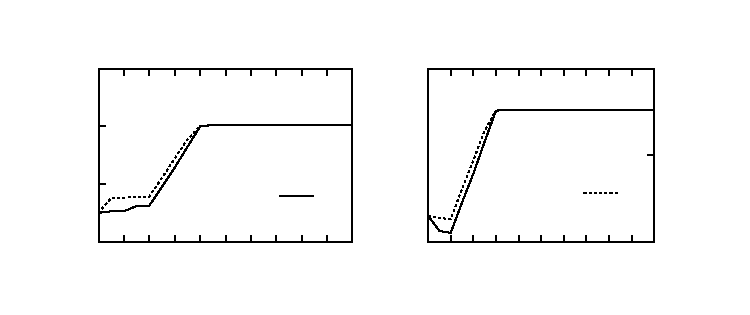
\includegraphics{CL2.pdf}}%
    \gplfronttext
  \end{picture}%
\endgroup
}}
{\resizebox{\textwidth}{!}{% GNUPLOT: LaTeX picture with Postscript
\begingroup
  \makeatletter
  \providecommand\color[2][]{%
    \GenericError{(gnuplot) \space\space\space\@spaces}{%
      Package color not loaded in conjunction with
      terminal option `colourtext'%
    }{See the gnuplot documentation for explanation.%
    }{Either use 'blacktext' in gnuplot or load the package
      color.sty in LaTeX.}%
    \renewcommand\color[2][]{}%
  }%
  \providecommand\includegraphics[2][]{%
    \GenericError{(gnuplot) \space\space\space\@spaces}{%
      Package graphicx or graphics not loaded%
    }{See the gnuplot documentation for explanation.%
    }{The gnuplot epslatex terminal needs graphicx.sty or graphics.sty.}%
    \renewcommand\includegraphics[2][]{}%
  }%
  \providecommand\rotatebox[2]{#2}%
  \@ifundefined{ifGPcolor}{%
    \newif\ifGPcolor
    \GPcolorfalse
  }{}%
  \@ifundefined{ifGPblacktext}{%
    \newif\ifGPblacktext
    \GPblacktexttrue
  }{}%
  % define a \g@addto@macro without @ in the name:
  \let\gplgaddtomacro\g@addto@macro
  % define empty templates for all commands taking text:
  \gdef\gplbacktext{}%
  \gdef\gplfronttext{}%
  \makeatother
  \ifGPblacktext
    % no textcolor at all
    \def\colorrgb#1{}%
    \def\colorgray#1{}%
  \else
    % gray or color?
    \ifGPcolor
      \def\colorrgb#1{\color[rgb]{#1}}%
      \def\colorgray#1{\color[gray]{#1}}%
      \expandafter\def\csname LTw\endcsname{\color{white}}%
      \expandafter\def\csname LTb\endcsname{\color{black}}%
      \expandafter\def\csname LTa\endcsname{\color{black}}%
      \expandafter\def\csname LT0\endcsname{\color[rgb]{1,0,0}}%
      \expandafter\def\csname LT1\endcsname{\color[rgb]{0,1,0}}%
      \expandafter\def\csname LT2\endcsname{\color[rgb]{0,0,1}}%
      \expandafter\def\csname LT3\endcsname{\color[rgb]{1,0,1}}%
      \expandafter\def\csname LT4\endcsname{\color[rgb]{0,1,1}}%
      \expandafter\def\csname LT5\endcsname{\color[rgb]{1,1,0}}%
      \expandafter\def\csname LT6\endcsname{\color[rgb]{0,0,0}}%
      \expandafter\def\csname LT7\endcsname{\color[rgb]{1,0.3,0}}%
      \expandafter\def\csname LT8\endcsname{\color[rgb]{0.5,0.5,0.5}}%
    \else
      % gray
      \def\colorrgb#1{\color{black}}%
      \def\colorgray#1{\color[gray]{#1}}%
      \expandafter\def\csname LTw\endcsname{\color{white}}%
      \expandafter\def\csname LTb\endcsname{\color{black}}%
      \expandafter\def\csname LTa\endcsname{\color{black}}%
      \expandafter\def\csname LT0\endcsname{\color{black}}%
      \expandafter\def\csname LT1\endcsname{\color{black}}%
      \expandafter\def\csname LT2\endcsname{\color{black}}%
      \expandafter\def\csname LT3\endcsname{\color{black}}%
      \expandafter\def\csname LT4\endcsname{\color{black}}%
      \expandafter\def\csname LT5\endcsname{\color{black}}%
      \expandafter\def\csname LT6\endcsname{\color{black}}%
      \expandafter\def\csname LT7\endcsname{\color{black}}%
      \expandafter\def\csname LT8\endcsname{\color{black}}%
    \fi
  \fi
  \setlength{\unitlength}{0.0500bp}%
  \begin{picture}(7200.00,3024.00)%
    \gplgaddtomacro\gplbacktext{%
      \csname LTb\endcsname%
      \put(814,704){\makebox(0,0)[r]{\strut{} 0}}%
      \put(814,1389){\makebox(0,0)[r]{\strut{} 10}}%
      \put(814,2074){\makebox(0,0)[r]{\strut{} 20}}%
      \put(814,2759){\makebox(0,0)[r]{\strut{} 30}}%
      \put(946,484){\makebox(0,0){\strut{} 0}}%
      \put(1190,484){\makebox(0,0){\strut{} 2}}%
      \put(1433,484){\makebox(0,0){\strut{} 4}}%
      \put(1677,484){\makebox(0,0){\strut{} 6}}%
      \put(1921,484){\makebox(0,0){\strut{} 8}}%
      \put(2165,484){\makebox(0,0){\strut{} 10}}%
      \put(2408,484){\makebox(0,0){\strut{} 12}}%
      \put(2652,484){\makebox(0,0){\strut{} 14}}%
      \put(2896,484){\makebox(0,0){\strut{} 16}}%
      \put(3139,484){\makebox(0,0){\strut{} 18}}%
      \put(3383,484){\makebox(0,0){\strut{} 20}}%
      \put(176,1731){\rotatebox{-270}{\makebox(0,0){\strut{}Inventory}}}%
      \put(2164,154){\makebox(0,0){\strut{}Time}}%
      \put(1921,2417){\makebox(0,0)[l]{\strut{}$\omega = 0.4$}}%
    }%
    \gplgaddtomacro\gplfronttext{%
    }%
    \gplgaddtomacro\gplbacktext{%
      \csname LTb\endcsname%
      \put(4109,484){\makebox(0,0){\strut{} 0}}%
      \put(4326,484){\makebox(0,0){\strut{} 2}}%
      \put(4544,484){\makebox(0,0){\strut{} 4}}%
      \put(4761,484){\makebox(0,0){\strut{} 6}}%
      \put(4978,484){\makebox(0,0){\strut{} 8}}%
      \put(5196,484){\makebox(0,0){\strut{} 10}}%
      \put(5413,484){\makebox(0,0){\strut{} 12}}%
      \put(5630,484){\makebox(0,0){\strut{} 14}}%
      \put(5847,484){\makebox(0,0){\strut{} 16}}%
      \put(6065,484){\makebox(0,0){\strut{} 18}}%
      \put(6282,484){\makebox(0,0){\strut{} 20}}%
      \put(6414,704){\makebox(0,0)[l]{\strut{} 10}}%
      \put(6414,1732){\makebox(0,0)[l]{\strut{} 20}}%
      \put(6414,2759){\makebox(0,0)[l]{\strut{} 30}}%
      \put(7051,1731){\rotatebox{-270}{\makebox(0,0){\strut{}Inventory}}}%
      \put(5195,154){\makebox(0,0){\strut{}Time}}%
    }%
    \gplgaddtomacro\gplfronttext{%
    }%
    \gplbacktext
    \put(0,0){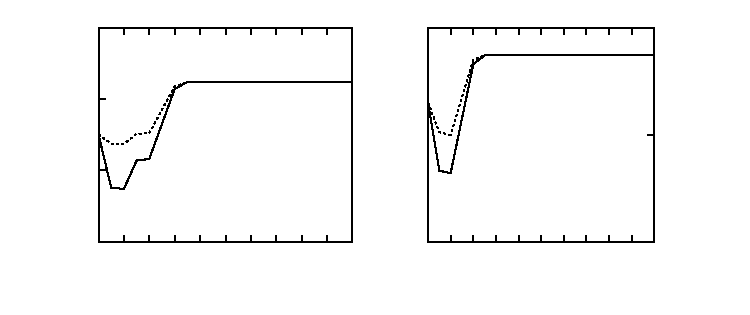
\includegraphics{CL4.pdf}}%
    \gplfronttext
  \end{picture}%
\endgroup
}}
{\resizebox{\textwidth}{!}{% GNUPLOT: LaTeX picture with Postscript
\begingroup
  \makeatletter
  \providecommand\color[2][]{%
    \GenericError{(gnuplot) \space\space\space\@spaces}{%
      Package color not loaded in conjunction with
      terminal option `colourtext'%
    }{See the gnuplot documentation for explanation.%
    }{Either use 'blacktext' in gnuplot or load the package
      color.sty in LaTeX.}%
    \renewcommand\color[2][]{}%
  }%
  \providecommand\includegraphics[2][]{%
    \GenericError{(gnuplot) \space\space\space\@spaces}{%
      Package graphicx or graphics not loaded%
    }{See the gnuplot documentation for explanation.%
    }{The gnuplot epslatex terminal needs graphicx.sty or graphics.sty.}%
    \renewcommand\includegraphics[2][]{}%
  }%
  \providecommand\rotatebox[2]{#2}%
  \@ifundefined{ifGPcolor}{%
    \newif\ifGPcolor
    \GPcolorfalse
  }{}%
  \@ifundefined{ifGPblacktext}{%
    \newif\ifGPblacktext
    \GPblacktexttrue
  }{}%
  % define a \g@addto@macro without @ in the name:
  \let\gplgaddtomacro\g@addto@macro
  % define empty templates for all commands taking text:
  \gdef\gplbacktext{}%
  \gdef\gplfronttext{}%
  \makeatother
  \ifGPblacktext
    % no textcolor at all
    \def\colorrgb#1{}%
    \def\colorgray#1{}%
  \else
    % gray or color?
    \ifGPcolor
      \def\colorrgb#1{\color[rgb]{#1}}%
      \def\colorgray#1{\color[gray]{#1}}%
      \expandafter\def\csname LTw\endcsname{\color{white}}%
      \expandafter\def\csname LTb\endcsname{\color{black}}%
      \expandafter\def\csname LTa\endcsname{\color{black}}%
      \expandafter\def\csname LT0\endcsname{\color[rgb]{1,0,0}}%
      \expandafter\def\csname LT1\endcsname{\color[rgb]{0,1,0}}%
      \expandafter\def\csname LT2\endcsname{\color[rgb]{0,0,1}}%
      \expandafter\def\csname LT3\endcsname{\color[rgb]{1,0,1}}%
      \expandafter\def\csname LT4\endcsname{\color[rgb]{0,1,1}}%
      \expandafter\def\csname LT5\endcsname{\color[rgb]{1,1,0}}%
      \expandafter\def\csname LT6\endcsname{\color[rgb]{0,0,0}}%
      \expandafter\def\csname LT7\endcsname{\color[rgb]{1,0.3,0}}%
      \expandafter\def\csname LT8\endcsname{\color[rgb]{0.5,0.5,0.5}}%
    \else
      % gray
      \def\colorrgb#1{\color{black}}%
      \def\colorgray#1{\color[gray]{#1}}%
      \expandafter\def\csname LTw\endcsname{\color{white}}%
      \expandafter\def\csname LTb\endcsname{\color{black}}%
      \expandafter\def\csname LTa\endcsname{\color{black}}%
      \expandafter\def\csname LT0\endcsname{\color{black}}%
      \expandafter\def\csname LT1\endcsname{\color{black}}%
      \expandafter\def\csname LT2\endcsname{\color{black}}%
      \expandafter\def\csname LT3\endcsname{\color{black}}%
      \expandafter\def\csname LT4\endcsname{\color{black}}%
      \expandafter\def\csname LT5\endcsname{\color{black}}%
      \expandafter\def\csname LT6\endcsname{\color{black}}%
      \expandafter\def\csname LT7\endcsname{\color{black}}%
      \expandafter\def\csname LT8\endcsname{\color{black}}%
    \fi
  \fi
  \setlength{\unitlength}{0.0500bp}%
  \begin{picture}(7200.00,3024.00)%
    \gplgaddtomacro\gplbacktext{%
      \csname LTb\endcsname%
      \put(814,704){\makebox(0,0)[r]{\strut{} 0}}%
      \put(814,1732){\makebox(0,0)[r]{\strut{} 10}}%
      \put(814,2759){\makebox(0,0)[r]{\strut{} 20}}%
      \put(946,484){\makebox(0,0){\strut{} 0}}%
      \put(1190,484){\makebox(0,0){\strut{} 2}}%
      \put(1433,484){\makebox(0,0){\strut{} 4}}%
      \put(1677,484){\makebox(0,0){\strut{} 6}}%
      \put(1921,484){\makebox(0,0){\strut{} 8}}%
      \put(2165,484){\makebox(0,0){\strut{} 10}}%
      \put(2408,484){\makebox(0,0){\strut{} 12}}%
      \put(2652,484){\makebox(0,0){\strut{} 14}}%
      \put(2896,484){\makebox(0,0){\strut{} 16}}%
      \put(3139,484){\makebox(0,0){\strut{} 18}}%
      \put(3383,484){\makebox(0,0){\strut{} 20}}%
      \put(176,1731){\rotatebox{-270}{\makebox(0,0){\strut{}Inventory}}}%
      \put(2164,154){\makebox(0,0){\strut{}Time}}%
      \put(1921,2245){\makebox(0,0)[l]{\strut{}$\omega = 0.8$}}%
    }%
    \gplgaddtomacro\gplfronttext{%
    }%
    \gplgaddtomacro\gplbacktext{%
      \csname LTb\endcsname%
      \put(4109,484){\makebox(0,0){\strut{} 0}}%
      \put(4326,484){\makebox(0,0){\strut{} 2}}%
      \put(4544,484){\makebox(0,0){\strut{} 4}}%
      \put(4761,484){\makebox(0,0){\strut{} 6}}%
      \put(4978,484){\makebox(0,0){\strut{} 8}}%
      \put(5196,484){\makebox(0,0){\strut{} 10}}%
      \put(5413,484){\makebox(0,0){\strut{} 12}}%
      \put(5630,484){\makebox(0,0){\strut{} 14}}%
      \put(5847,484){\makebox(0,0){\strut{} 16}}%
      \put(6065,484){\makebox(0,0){\strut{} 18}}%
      \put(6282,484){\makebox(0,0){\strut{} 20}}%
      \put(6414,704){\makebox(0,0)[l]{\strut{} 0}}%
      \put(6414,1389){\makebox(0,0)[l]{\strut{} 10}}%
      \put(6414,2074){\makebox(0,0)[l]{\strut{} 20}}%
      \put(6414,2759){\makebox(0,0)[l]{\strut{} 30}}%
      \put(7051,1731){\rotatebox{-270}{\makebox(0,0){\strut{}Inventory}}}%
      \put(5195,154){\makebox(0,0){\strut{}Time}}%
    }%
    \gplgaddtomacro\gplfronttext{%
    }%
    \gplbacktext
    \put(0,0){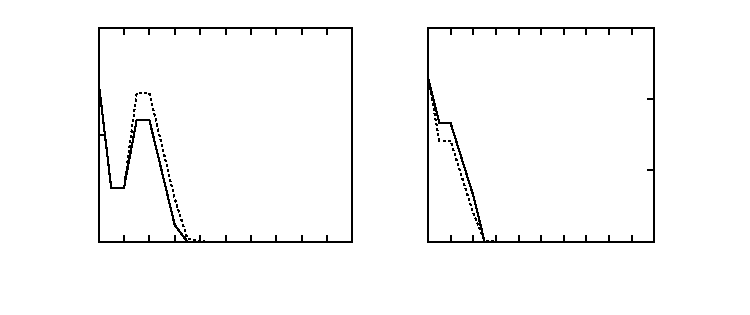
\includegraphics{CL8.pdf}}%
    \gplfronttext
  \end{picture}%
\endgroup
}}
\caption{Comparison of Closed-loop response using a pure tracking
  stage cost and a multiobjective stage cost for different values of
  $\omega$}% ($\omega = 0.2$: top, $\omega = 0.4$: 
%middle and $\omega = 0.8$: bottom)}
\label{fig:esc:CL}
\end{figure*}

In Table \ref{tab:esc:CL}, we compare the economic cost incurred in using
the three controllers: (i) Multiobjective MPC $\ell(x,u;z_t)$, (ii)
Economic MPC $\ell_E(x,u)$ and (iii) Tracking MPC to the steady state
of the multiobjective MPC $\ell_T(x,u,z_s)$. 

\begin{table}[h]
\caption{Economic cost of implementing MPC}
\label{tab:esc:CL}
\centering
\begin{tabular}{cccc}\toprule
$\omega$ & Multiobjective$ _{ \times 10^{4}}$ & Tracking$ _{ \times 10^{4}}$ & Economic$ _{ \times 10^{4}}$ \\
%& \hfill$ _{ \times 10^{4}}$ & \hfill$_{\times 10^{4}}$ &\hfill
%$_{\times 10^{4}}$ \\
\midrule
0 & 4.43 & 4.43 & infeasible \\
0.2 & 4.02 & 4.06 & infeasible \\
0.4 & 3.56 & 3.63 & infeasible \\
%0.6 & 2.73 & 2.74 & 2.74 (stabilizes origin) \\
0.8 & 2.27 & 2.27 & 2.27 \\
1.0 & 2.27 & 2.27 & 2.27 \\
\bottomrule
\end{tabular}
\end{table}

From Figure \ref{fig:esc:CL} and Table \ref{tab:esc:CL}, we can
observe that when economic information is available to the controller,
it follows an economically attractive transient while stabilizing the
steady sate. Hence, the advantage of the multiobjective formulation as
compared to a pure tracking formulation (risk averse) is that the
steady state can be stabilized via a cost effective transient. The
advantage of the multiobjective formulation as compared to a pure
economic formulation (risk seeking) is that the multiobjective
formulation allows a larger region of attraction. For instance, if we
wished to stabilize a set-point $z_p = (x_p,u_p)$ using economic MPC,
one way to do it would be to change the constraint set $x_p \leq Ix \leq
\bar{x}$, so that the solution to \eqref{eq:esc:SSx} is
$x_p$. However, as observed in Table \ref{tab:esc:CL}, by using the
multiobjective formulation, we could stabilize a larger space of
initial states. 

\section{Multiechelon, multiproduct supply chain}
\label{sec:multi}
We follow the design procedure presented in the previous section to
develop a stabilizing MPC for an 8-node supply chain. The supply chain
studied is shown in Figure \ref{fig:esc:lssc}. It consists of a
manufacturing facility that can produce 2 products -- A and B. The
manufacturing facility is node $M1$. Node $M1$ supplies products to
nodes $D1$ and $D2$, which are distribution centers. Node $M1$ also
sells directly to retailer $R5$. Distributor $D1$ sells products to
retailers $R1$ and $R2$, while $D2$ serves retailers $R3$ and $R4$. 


\begin{figure}
\centering
\scriptsize
{\resizebox{0.5\textwidth}{!}{\begin{picture}(0,0)%
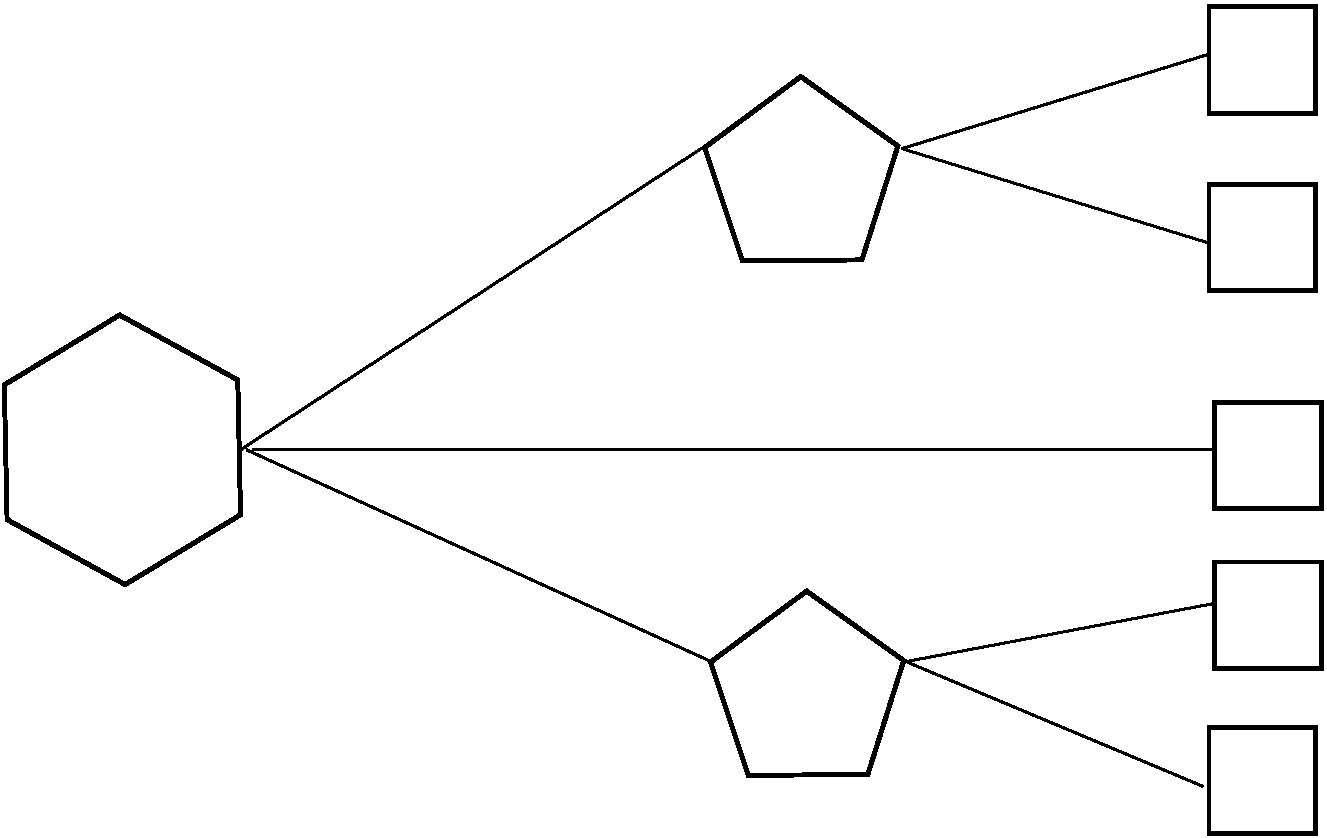
\includegraphics{lssc.pdf}%
\end{picture}%
\setlength{\unitlength}{4144sp}%
%
\begingroup\makeatletter\ifx\SetFigFont\undefined%
\gdef\SetFigFont#1#2#3#4#5{%
  \reset@font\fontsize{#1}{#2pt}%
  \fontfamily{#3}\fontseries{#4}\fontshape{#5}%
  \selectfont}%
\fi\endgroup%
\begin{picture}(10101,6366)(1363,-5719)
\put(10801,164){\makebox(0,0)[lb]{\smash{{\SetFigFont{17}{20.4}{\familydefault}{\mddefault}{\updefault}{\color[rgb]{0,0,0}$R1$}%
}}}}
\put(2071,-2851){\makebox(0,0)[lb]{\smash{{\SetFigFont{17}{20.4}{\familydefault}{\mddefault}{\updefault}{\color[rgb]{0,0,0}$M1$}%
}}}}
\put(7246,-736){\makebox(0,0)[lb]{\smash{{\SetFigFont{17}{20.4}{\familydefault}{\mddefault}{\updefault}{\color[rgb]{0,0,0}$D1$}%
}}}}
\put(7291,-4741){\makebox(0,0)[lb]{\smash{{\SetFigFont{17}{20.4}{\familydefault}{\mddefault}{\updefault}{\color[rgb]{0,0,0}$D2$}%
}}}}
\put(10801,-5371){\makebox(0,0)[lb]{\smash{{\SetFigFont{17}{20.4}{\familydefault}{\mddefault}{\updefault}{\color[rgb]{0,0,0}$R4$}%
}}}}
\put(10846,-4111){\makebox(0,0)[lb]{\smash{{\SetFigFont{17}{20.4}{\familydefault}{\mddefault}{\updefault}{\color[rgb]{0,0,0}$R3$}%
}}}}
\put(10891,-2896){\makebox(0,0)[lb]{\smash{{\SetFigFont{17}{20.4}{\familydefault}{\mddefault}{\updefault}{\color[rgb]{0,0,0}$R5$}%
}}}}
\put(10801,-1231){\makebox(0,0)[lb]{\smash{{\SetFigFont{17}{20.4}{\familydefault}{\mddefault}{\updefault}{\color[rgb]{0,0,0}$R2$}%
}}}}
\end{picture}%
}}
\caption{Multiproduct, Multiechelon supply chain studied}
\label{fig:esc:lssc}
\end{figure}

The production time for product $A$ is 2 time units while that for product $B$ is 3 time units. We assume that the facility $M1$ can start producing either batch at every sampling time. 

In Table \ref{tab:esc:translead}, we list the shipment delay between
the nodes. We assume that the customer demand is normally distributed
around the nominal demand. In Table \ref{tab:esc:dem}, we list the
nominal demand and the variance  of the demand for each product at the
retailer nodes. The first entry in Table \ref{tab:esc:dem} is the
nominal demand while the second entry is the variance of the
demand. In the simulation examples, we assumed zero demand if the
demand realization is negative. 

\begin{table}
\caption{Transportation lead times}
\label{tab:esc:translead}
\centering
\begin{tabular}{cccccccc}\toprule
& $D1$ & $D2$  & $R1$ & $R2$ & $R3$ & $R4$ & $R5$ \\
\midrule
$M1$ &2&1& & & & &4\\
$D1$ & & &1&1& & & \\
$D2$ & & & & &2&1& \\
\bottomrule
\end{tabular}
\end{table}
\begin{table}
\caption{Nominal demand and variance of demand}
\centering
\begin{tabular}{cccccc}\toprule
\label{tab:esc:dem}
 &$R1$&$R2$&$R3$&$R4$&$R5$\\
\midrule
$A$&(3.0,1.1)&(4.5,1.3)&(5.0,1.1)&(2.0,1.2)&(4.0,1.4)\\
$B$&(4.2,1.3)&(3.1,1.4)&(1.4,1.1)&(2.5,1.1)&(4.2,1.4)\\
\bottomrule
\end{tabular}
\end{table}

The target inventory is chosen as the amount of product to be
maintained to meet nominal customer demands for the longest delay in
the supply chain. In this example, because the longest delay is four time
units (between $M1$ and $R5$), the target inventory at each retailer
node was four times the nominal demand. For the upstream nodes, the
target inventory is four times the sum of the nominal demands at all
the retailers served by that node.  The target inventories are
listed in the Table \ref{tab:esc:targinv}.  The target backorder at
all nodes are zero. At each node, we also assign a capacity
constraint. The capacity constraint is the total amount of product
that can be stored in the node. The capacity constraint is listed in
Table \ref{tab:esc:constraints}.   

The economic  cost at a node $i$ is:
\[ \ell_E(x_i,u_i) =  \sum_{j \in \set{A,B}}h_{i,j} \Inv_{i,j} + g_{i,j} \BO_{i,j} + s_{i,j} S_{i,j} + o_{i,j} O_{i,j} \]
in which $h_{i,j}$ is the inventory holding cost, $g_{i,j}$ is the backorder penalty, $s_{i,j}$ is the shipping cost and $o_{i,j}$ is the ordering cost at node $i$ for product $j$.  The variable $\BO_{i,j}$ is the total backorder at the node. For the manufacturing node $o_{i,j}$ represents the production cost. The economic cost parameters are listed in Tables \ref{tab:esc:state_economic} and Table \ref{tab:esc:input_economic} (the first entry is for product $A$, while the second entry is for product $B$).  The ordering cost is $1$ per unit except at $R5$ where it is $0.5$ per unit. The production cost of $A$ is 10 per unit while that for $B$ is 4 per unit.


The tracking objective function is the sum of squares of the deviation from the target. That is:
\[\ell_T(x_i,u_i) = (x_i-x_{i,t})'Q_i( x_i-x_{i,t}) + (u_i-u_{i,t})'R_i(u_i-u_{i,t})\]

The matrix $R_i$ was $0.1I$, $I$ being the identity matrix. The matrix
$Q_i$ was $Q_i = \text{diag}(1,10,1,10)$. Recall that the definition
of state for node $i$ is $\begin{bmatrix} \Inv_{i,A} & \BO_{i,A} &
  \Inv_{i,B} &   \BO_{i,B} \end{bmatrix}'$. 

\begin{table}
\caption{Target inventories}
\label{tab:esc:targinv}
\centering
\begin{tabular}{ccccccccc}\toprule
& $M1$ & $D1$ & $D2$  & $R1$ & $R2$ & $R3$ & $R4$ & $R5$ \\
\midrule
$A$&70&30  &24   &12  &18  &20 &8 &16\\
$B$&61&29.2&15.6 &16.8&12.4&5.6&10&16.8 \\
\bottomrule
\end{tabular}
\end{table}
\begin{table}
\caption{Capacity constraints}
\label{tab:esc:constraints}
\centering
\begin{tabular}{ccccccccc}\toprule
& $M1$ & $D1$ & $D2$  & $R1$ & $R2$ & $R3$ & $R4$ & $R5$ \\
\midrule
$\Inv_A+\Inv_B$&140&80  &50   &40  &40  &30 &25 &45\\
\bottomrule
\end{tabular}
\caption{State economic costs (per unit)}
\label{tab:esc:state_economic}
\centering
\begin{tabular}{ccccccccc}\toprule
& $M1$ & $D1$ & $D2$  & $R1$ & $R2$ & $R3$ & $R4$ & $R5$ \\
\midrule
Inventory holding &1&1  &1   &1  &1  &1 &1 &1\\
Back-order &10&10&10 &10&10&10&10&10 \\
\bottomrule
\end{tabular}
\end{table}
\begin{table}
\caption{Input economic costs (per unit)}
\label{tab:esc:input_economic}
\centering
\begin{tabular}{cccccccc}\toprule
& $D1$ & $D2$  & $R1$ & $R2$ & $R3$ & $R4$ & $R5$ \\
\midrule
$M1$ &(4,2)&(1,2)& & & & &(5,4)\\
$D1$ & & &(1,1)&(1,1)& & & \\
$D2$ & & & & &(2,2)&(1.5,1.5)& \\
\bottomrule
\end{tabular}
\end{table}

We choose $\omega  = 0.4$ in the stage cost $\ell(x,u)$ given by
\eqref{eq:esc:ell} with the economic and tracking functions defined
using the parameters listed in the tables. The steady-state problem
\eqref{eq:SS} is solved for the nominal demand. The online MPC problem
is given by \eqref{eq:PN_equality1}.  The prediction horizon is 15
days. We simulate the supply chain for 50 days using a stochastic
demand signal. For making the predictions, we make a demand forecast
$\bd$. We assume that we have perfect demand information for three
days. For the remainder of the horizon, the demand forecast is set to the
nominal demand. The initial inventories of the nodes is given in Table
\ref{tab:esc:initial}. 
\begin{table}
\caption{Initial inventories}
\label{tab:esc:initial}
\centering
\begin{tabular}{ccccccccc}\toprule
& $M1$ & $D1$ & $D2$  & $R1$ & $R2$ & $R3$ & $R4$ & $R5$ \\
\midrule
$A$                      &63   &14   &24   &0 &2.1  &3.1  &3.1&0 \\
$B$                      &40   &12   &7    &0 &1.2  &1.2  &0  &5.2   \\
\bottomrule
\end{tabular}
\end{table}
All the backorders are zero, and the inputs are at their steady state
at the beginning of the simulation.

\begin{xalignat}{2}
\label{eq:PN_equality1}
\mathbb{P}_N(x;\bd) :& \min_{\bu}{V_N(\bu;x)} & \nonumber \\
&\text{s.t.~} x(j+1) = Ax(j) + Bu(j) +B_dd(j), & j \in
\mathbb{I}_{0:N-1} \nonumber \\
&x(j) \in \mathbb{X}& j \in \mathbb{I}_{0:N-1} \\
&u(j) \in \mathbb{U}& j \in \mathbb{I}_{0:N-1} \nonumber \\
&x(N) = x_s & \nonumber
\end{xalignat}

In Figure \ref{fig:esc:bullwhip}, we plot the variance of the orders
placed by a node and compare it with the variance of the orders
arriving at the node. It has been found that classical control methods
can often increase the variance of orders placed by the node when
compared to the variance of the incoming orders as we move upstream in
the supply chain. This effect is called the bullwhip effect
\cite{lee:padmanabhan:whang:1997,lee:padmanabhan:whang:1997b}. From
Figure \ref{fig:esc:bullwhip}, it is clear that the centralized model
predictive controller does not show a bullwhip effect. As has been noted in previous studies \cite{moyaux:chaib-draa:damours:2007},the knowledge of the entire supply chain dynamics along with better forecasts results in the better solution (no bullwhip effect).


In Figure \ref{fig:esc:Order}, we plot the orders placed by the MPC
controller and the corresponding inventory and backorder profile in response to
demands of product $A$ at Retailer $R3$. Note that the steady state
for product $A$ is 7.93 units.


\begin{figure}
\centering
\scriptsize
{\resizebox{1\textwidth}{!}{% GNUPLOT: LaTeX picture with Postscript
\begingroup
  \makeatletter
  \providecommand\color[2][]{%
    \GenericError{(gnuplot) \space\space\space\@spaces}{%
      Package color not loaded in conjunction with
      terminal option `colourtext'%
    }{See the gnuplot documentation for explanation.%
    }{Either use 'blacktext' in gnuplot or load the package
      color.sty in LaTeX.}%
    \renewcommand\color[2][]{}%
  }%
  \providecommand\includegraphics[2][]{%
    \GenericError{(gnuplot) \space\space\space\@spaces}{%
      Package graphicx or graphics not loaded%
    }{See the gnuplot documentation for explanation.%
    }{The gnuplot epslatex terminal needs graphicx.sty or graphics.sty.}%
    \renewcommand\includegraphics[2][]{}%
  }%
  \providecommand\rotatebox[2]{#2}%
  \@ifundefined{ifGPcolor}{%
    \newif\ifGPcolor
    \GPcolorfalse
  }{}%
  \@ifundefined{ifGPblacktext}{%
    \newif\ifGPblacktext
    \GPblacktexttrue
  }{}%
  % define a \g@addto@macro without @ in the name:
  \let\gplgaddtomacro\g@addto@macro
  % define empty templates for all commands taking text:
  \gdef\gplbacktext{}%
  \gdef\gplfronttext{}%
  \makeatother
  \ifGPblacktext
    % no textcolor at all
    \def\colorrgb#1{}%
    \def\colorgray#1{}%
  \else
    % gray or color?
    \ifGPcolor
      \def\colorrgb#1{\color[rgb]{#1}}%
      \def\colorgray#1{\color[gray]{#1}}%
      \expandafter\def\csname LTw\endcsname{\color{white}}%
      \expandafter\def\csname LTb\endcsname{\color{black}}%
      \expandafter\def\csname LTa\endcsname{\color{black}}%
      \expandafter\def\csname LT0\endcsname{\color[rgb]{1,0,0}}%
      \expandafter\def\csname LT1\endcsname{\color[rgb]{0,1,0}}%
      \expandafter\def\csname LT2\endcsname{\color[rgb]{0,0,1}}%
      \expandafter\def\csname LT3\endcsname{\color[rgb]{1,0,1}}%
      \expandafter\def\csname LT4\endcsname{\color[rgb]{0,1,1}}%
      \expandafter\def\csname LT5\endcsname{\color[rgb]{1,1,0}}%
      \expandafter\def\csname LT6\endcsname{\color[rgb]{0,0,0}}%
      \expandafter\def\csname LT7\endcsname{\color[rgb]{1,0.3,0}}%
      \expandafter\def\csname LT8\endcsname{\color[rgb]{0.5,0.5,0.5}}%
    \else
      % gray
      \def\colorrgb#1{\color{black}}%
      \def\colorgray#1{\color[gray]{#1}}%
      \expandafter\def\csname LTw\endcsname{\color{white}}%
      \expandafter\def\csname LTb\endcsname{\color{black}}%
      \expandafter\def\csname LTa\endcsname{\color{black}}%
      \expandafter\def\csname LT0\endcsname{\color{black}}%
      \expandafter\def\csname LT1\endcsname{\color{black}}%
      \expandafter\def\csname LT2\endcsname{\color{black}}%
      \expandafter\def\csname LT3\endcsname{\color{black}}%
      \expandafter\def\csname LT4\endcsname{\color{black}}%
      \expandafter\def\csname LT5\endcsname{\color{black}}%
      \expandafter\def\csname LT6\endcsname{\color{black}}%
      \expandafter\def\csname LT7\endcsname{\color{black}}%
      \expandafter\def\csname LT8\endcsname{\color{black}}%
    \fi
  \fi
  \setlength{\unitlength}{0.0500bp}%
  \begin{picture}(7200.00,5040.00)%
    \gplgaddtomacro\gplbacktext{%
      \csname LTb\endcsname%
      \put(946,846){\makebox(0,0)[r]{\strut{} 0}}%
      \put(946,1828){\makebox(0,0)[r]{\strut{} 0.5}}%
      \put(946,2811){\makebox(0,0)[r]{\strut{} 1}}%
      \put(946,3793){\makebox(0,0)[r]{\strut{} 1.5}}%
      \put(946,4775){\makebox(0,0)[r]{\strut{} 2}}%
      \put(2223,714){\rotatebox{-45}{\makebox(0,0)[l]{\strut{}R1}}}%
      \put(3368,714){\rotatebox{-45}{\makebox(0,0)[l]{\strut{}R5}}}%
      \put(4513,714){\rotatebox{-45}{\makebox(0,0)[l]{\strut{}D1}}}%
      \put(5658,714){\rotatebox{-45}{\makebox(0,0)[l]{\strut{}D2}}}%
      \put(176,2810){\rotatebox{-270}{\makebox(0,0){\strut{}Standard deviation of Orders}}}%
    }%
    \gplgaddtomacro\gplfronttext{%
      \csname LTb\endcsname%
      \put(3085,173){\makebox(0,0)[r]{\strut{}Incoming}}%
      \csname LTb\endcsname%
      \put(4996,173){\makebox(0,0)[r]{\strut{}MPC}}%
    }%
    \gplbacktext
    \put(0,0){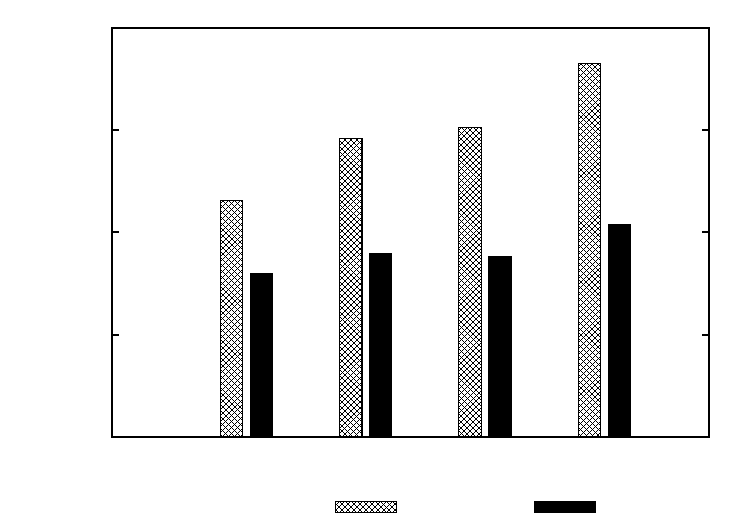
\includegraphics{bullwhip.pdf}}%
    \gplfronttext
  \end{picture}%
\endgroup
}}
\caption{Bullwhip effect using MPC}
\label{fig:esc:bullwhip}
\end{figure}
\begin{figure}
\scriptsize
{\resizebox{1\textwidth}{!}{% GNUPLOT: LaTeX picture with Postscript
\begingroup
  \makeatletter
  \providecommand\color[2][]{%
    \GenericError{(gnuplot) \space\space\space\@spaces}{%
      Package color not loaded in conjunction with
      terminal option `colourtext'%
    }{See the gnuplot documentation for explanation.%
    }{Either use 'blacktext' in gnuplot or load the package
      color.sty in LaTeX.}%
    \renewcommand\color[2][]{}%
  }%
  \providecommand\includegraphics[2][]{%
    \GenericError{(gnuplot) \space\space\space\@spaces}{%
      Package graphicx or graphics not loaded%
    }{See the gnuplot documentation for explanation.%
    }{The gnuplot epslatex terminal needs graphicx.sty or graphics.sty.}%
    \renewcommand\includegraphics[2][]{}%
  }%
  \providecommand\rotatebox[2]{#2}%
  \@ifundefined{ifGPcolor}{%
    \newif\ifGPcolor
    \GPcolorfalse
  }{}%
  \@ifundefined{ifGPblacktext}{%
    \newif\ifGPblacktext
    \GPblacktexttrue
  }{}%
  % define a \g@addto@macro without @ in the name:
  \let\gplgaddtomacro\g@addto@macro
  % define empty templates for all commands taking text:
  \gdef\gplbacktext{}%
  \gdef\gplfronttext{}%
  \makeatother
  \ifGPblacktext
    % no textcolor at all
    \def\colorrgb#1{}%
    \def\colorgray#1{}%
  \else
    % gray or color?
    \ifGPcolor
      \def\colorrgb#1{\color[rgb]{#1}}%
      \def\colorgray#1{\color[gray]{#1}}%
      \expandafter\def\csname LTw\endcsname{\color{white}}%
      \expandafter\def\csname LTb\endcsname{\color{black}}%
      \expandafter\def\csname LTa\endcsname{\color{black}}%
      \expandafter\def\csname LT0\endcsname{\color[rgb]{1,0,0}}%
      \expandafter\def\csname LT1\endcsname{\color[rgb]{0,1,0}}%
      \expandafter\def\csname LT2\endcsname{\color[rgb]{0,0,1}}%
      \expandafter\def\csname LT3\endcsname{\color[rgb]{1,0,1}}%
      \expandafter\def\csname LT4\endcsname{\color[rgb]{0,1,1}}%
      \expandafter\def\csname LT5\endcsname{\color[rgb]{1,1,0}}%
      \expandafter\def\csname LT6\endcsname{\color[rgb]{0,0,0}}%
      \expandafter\def\csname LT7\endcsname{\color[rgb]{1,0.3,0}}%
      \expandafter\def\csname LT8\endcsname{\color[rgb]{0.5,0.5,0.5}}%
    \else
      % gray
      \def\colorrgb#1{\color{black}}%
      \def\colorgray#1{\color[gray]{#1}}%
      \expandafter\def\csname LTw\endcsname{\color{white}}%
      \expandafter\def\csname LTb\endcsname{\color{black}}%
      \expandafter\def\csname LTa\endcsname{\color{black}}%
      \expandafter\def\csname LT0\endcsname{\color{black}}%
      \expandafter\def\csname LT1\endcsname{\color{black}}%
      \expandafter\def\csname LT2\endcsname{\color{black}}%
      \expandafter\def\csname LT3\endcsname{\color{black}}%
      \expandafter\def\csname LT4\endcsname{\color{black}}%
      \expandafter\def\csname LT5\endcsname{\color{black}}%
      \expandafter\def\csname LT6\endcsname{\color{black}}%
      \expandafter\def\csname LT7\endcsname{\color{black}}%
      \expandafter\def\csname LT8\endcsname{\color{black}}%
    \fi
  \fi
  \setlength{\unitlength}{0.0500bp}%
  \begin{picture}(7200.00,3024.00)%
    \gplgaddtomacro\gplbacktext{%
      \csname LTb\endcsname%
      \put(594,946){\makebox(0,0)[r]{\strut{} 0}}%
      \put(594,2155){\makebox(0,0)[r]{\strut{} 10}}%
      \put(828,484){\makebox(0,0){\strut{} 0}}%
      \put(1339,484){\makebox(0,0){\strut{} 10}}%
      \put(1850,484){\makebox(0,0){\strut{} 20}}%
      \put(2361,484){\makebox(0,0){\strut{} 30}}%
      \put(2872,484){\makebox(0,0){\strut{} 40}}%
      \put(3383,484){\makebox(0,0){\strut{} 50}}%
      \put(2054,154){\makebox(0,0){\strut{}Time}}%
    }%
    \gplgaddtomacro\gplfronttext{%
      \csname LTb\endcsname%
      \put(2396,2586){\makebox(0,0)[r]{\strut{}Inventory}}%
      \csname LTb\endcsname%
      \put(2396,2366){\makebox(0,0)[r]{\strut{}Backorder}}%
    }%
    \gplgaddtomacro\gplbacktext{%
      \csname LTb\endcsname%
      \put(4201,484){\makebox(0,0){\strut{} 0}}%
      \put(4661,484){\makebox(0,0){\strut{} 10}}%
      \put(5121,484){\makebox(0,0){\strut{} 20}}%
      \put(5582,484){\makebox(0,0){\strut{} 30}}%
      \put(6042,484){\makebox(0,0){\strut{} 40}}%
      \put(6502,484){\makebox(0,0){\strut{} 50}}%
      \put(6634,704){\makebox(0,0)[l]{\strut{} 0}}%
      \put(6634,1732){\makebox(0,0)[l]{\strut{} 10}}%
      \put(6634,2759){\makebox(0,0)[l]{\strut{} 20}}%
      \put(5305,154){\makebox(0,0){\strut{}Time}}%
    }%
    \gplgaddtomacro\gplfronttext{%
      \csname LTb\endcsname%
      \put(5779,2586){\makebox(0,0)[r]{\strut{}Customer demand}}%
      \csname LTb\endcsname%
      \put(5779,2366){\makebox(0,0)[r]{\strut{}Orders placed}}%
    }%
    \gplbacktext
    \put(0,0){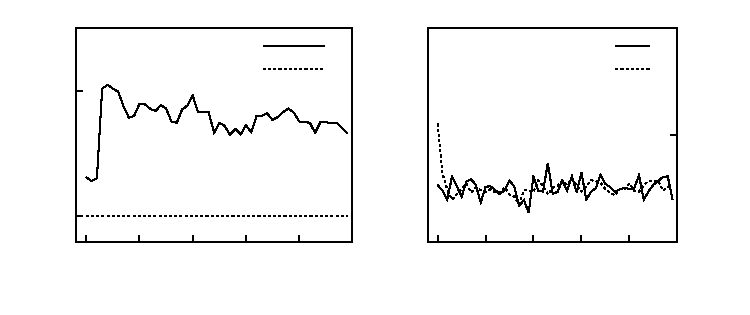
\includegraphics{R3.pdf}}%
    \gplfronttext
  \end{picture}%
\endgroup
}}
\caption{State and Input  profile at $R3$ using MPC}
\label{fig:esc:Order}
\end{figure}




In Table \ref{tab:esc:avgA}, we list the average inventory at each
node for products $A$. and the steady-state inventory for $A$.  The
data in the table highlights the inherent robustness of MPC. Although
the MPC is designed for the nominal demand (the steady state and the
terminal condition are calculated based on the nominal demand); we
observe that the controller was able to reject deviations around the
nominal demand.

\begin{table}[h]
\caption{Average inventory for Product-A}
\label{tab:esc:avgA}
\begin{center}
\begin{tabular}{cccccccccc}\toprule
 &$M1$&$D1$&$D2$&$R1$&$R2$&$R3$&$R4$&$R5$\\ \midrule
MPC&58.0&17.5&12.4&0.34&5.43&7.71&0.26&3.44\\ 
Steady state&57.9&17.9&11.9&0 &5.93&7.93&0&3.93\\
\bottomrule 
\end{tabular}
\end{center}
\end{table}

\section{Integration of scheduling and control}
\label{sec:multi:integration}
In the previous section, the manufacturing facility could start a
batch of either product at every time. In this section, we use the
following model for the manufacturing facility: There is one unit in
the facility that can carry out both the tasks of producing $A$ and
$B$ from raw-materials. The batch time to make $A$ is two sampling
times while that to make $B$ is 3 sampling times. In addition, there
is a 1 period changeover time whenever a change of batch from that of
$A$ to $B$ has to be made.  

We model the manufacturing facility using the State Task Network
approach\cite{shah:pantelides:sargent:1993}, though the same approach can be followed using any discrete-time scheduling model \cite{mendez:cerda:grossmann:harjunkoski:fahl:2006,maravelias:2012}.  A single unit $U$ in
$M1$ can perform two tasks $\text{TA},\text{TB}$ that produce final
products $A,B$ respectively.  We denote the set $\mathbf{I} =
\set{\text{TA},\text{TB}}$, the production lead times by the set
$\tau_{P}(i)$ and the changeover times from task $i \in \mathbf{I}$ to
task $i' \in \mathbf{I}, i' \neq i$ by $\tau_{C}(i,i')$. There is an
economic cost associated with starting a batch as well as changeovers.
For ease of presentation we use four binary variables $W_{i,t}, Z_{i,i',t}, Y_{i,t}, X_{i,t}$, to model that  (i) only one task can be running in the unit at any given time, and (ii) if a changeover from one task to another has to take place then we need to wait for $\tau_{C}(i,i')$ time period. The binary variable $W_{i,t}=1$ denotes that a batch of $i$ has started at time $t$.  The binary variable $Z(i,i',t) = 1$ denotes that a changeover has  been made at time $t$ from $i \rightarrow i'$. The binary variable $Y_{i,t} = 1$ if the task $i$ is being carried out at time $t$, while the binary variable $X_{i,t}$ is 1 if the last task to be carried out in the unit was $i$.  The scheduling constraints are enforced by the following inequalities:

\begin{alignat}{2}
&\sum_{i\in \mathbf{I}}\sum_{t' = t-\tau_i+1}^{t}W_{i,t'}+\sum_{i' \in
 \mathbf{I} \atop i' \neq i}\sum_{t'=t-\tau_{C}(i,i')+1}^{t}
Z_{i,i',t'} \leq 1 & \forall t \nonumber \\ 
&\sum_{t' = t-\tau_i+1}^{t} W_{i,t'} = Y_{i,t} & \forall t, \forall i
\in \mathbf{I} \nonumber\\
&X_{i,t} \geq Y_{i,t} & \forall t, \forall i \in \mathbf{I} \nonumber\\
&\sum_{i \in \mathbf{I}}X_{i,t} = 1 & \forall
t  \label{eq:esc:assign}\\ 
&Z_{i,i',t} \leq X_{i,t-1} &\forall t, \forall i \in \mathbf{I}, i' \in
\mathbf{I}, i' \neq i \nonumber\\
&Z_{i,i',t} \leq X_{i',t} &\forall t, \forall i \in \mathbf{I}, i' \in
\mathbf{I}, i'\neq i \nonumber \\
&Z_{i,i',t} \geq X_{i,t-1}+X_{i',t}-1 &\forall t, \forall i \in \mathbf{I}, i' \in
\mathbf{I}, i' \neq i \nonumber
\end{alignat}

The batch size is given by $B_{i,t}$ and is constrained by
\begin{equation}
\label{eq:esc:bts}
W_{i,t}\underbar{B}_i \leq B_{i,t} \leq W_{i,t}\bar{B}_i
\end{equation}
 in which $\underbar{B}_i,\bar{B}_i$ are the minimum and maximum batchsizes. 
 
 The dynamics of the manufacturing node for the inventory of $A$ is now
 \begin{equation}
 \label{eq:esc:invam}
 \Inv_{A,\text{M1},t+1} = \Inv _{A,\text{M1},t} + B_{A,t-\tau_{P}(\text{TA})} - \sum_{i \in \set{D1,D2,R5}}S_{A, i,t}
 \end{equation}
 Similarly, the dynamics for inventory of $B$ at the node also
 changes. The dynamic equations for the rest of the supply chain
 remains the same.  
 
 Following the procedure outlined in
 \cite{subramanian:maravelias:rawlings:2012}, the supply chain
 dynamics with the integrated scheduling model can be converted into
 the state space form \eqref{eq:model}. 
The terminal conditions used in \eqref{eq:PN_equality} and
\eqref{eq:PN_region} ensure that the supply chain is able to respond
to the nominal demand at the end of the optimization horizon
indefinitely. For example, the steady state is chosen so that the
supply chain can meet the customer demands and stay at the same
state. Hence, the terminal conditions help us identify a suboptimal
infinite horizon control sequence. When the system moves to the
successor state after implementing the first input move in the
suboptimal infinite horizon control sequence, we have a readily
available candidate input sequence for the successor state. Thus, the
terminal conditions ensure recursive feasibility. In the
case of the scheduling problem, we find a periodic steady state. We
define $N_p$ as the period, and solve the following optimization
problem \eqref{eq:esc:Pp}, in which we ensure that the system returns
to the same state every $N_p$ sampling times. The periodic schedule is
another example of an infinite horizon suboptimal input sequence. For
this problem, many choices of the period $N_p$ exists. We choose
$N_p=24$. For a general scheduling model cast in the state space form,
a periodic schedule may not exist. An avenue of future work is to
find suitable terminal constraints for such cases.

 We solve the integrated scheduling and control problem only for the economic objective. The cost associated with starting a batch of TA as 10, while that of TB was 6. The cost of changeover from TA to TB was 10 while that of TB to TA was 5. 
 
 
\begin{alignat}{2}
\label{eq:esc:Pp}
\mathbb{P}_p:& \min_{\bu,x(0)}{\sum_{i=0}^{N_p-1}\ell_E(x(i),u(i),d_s(i))}& \nonumber \\
&\text{s.t.~} x(i+1) = Ax(i) + Bu(i)+B_dd_s(i),&i = \mathbb{I}_{0:N_p-1} \\
&(x(i),u(i)) \in \mathbb{Z}&i = \mathbb{I}_{0:N_p-1}\nonumber\\
& x(0) = x(N_p)& \nonumber
\end{alignat}
in which the set $\mathbb{Z}$ is the combined state-input constraints that consists of the supply chain constraints from the previous section and the assignment constraints \eqref{eq:esc:assign} and \eqref{eq:esc:bts}. 

 We denote the solution to
\eqref{eq:esc:Pp} by $(\mathbf{u}_p^0,x(0)_p^0)$.
The solution to \eqref{eq:esc:Pp} gives us the periodic state-profile
\begin{equation}
\label{eq:esc:Xperiodic}
\mathbb{X}_p =  \set {x^0_p(0),x(1;x^0_p(0),\bu_p^0,\bd_s),\ldots,x(N_p;x^0_p(0),\bu_p^0,\bd_s) }
\end{equation}
In Figure \ref{fig:esc:gantt_ss}, we show the Gantt chart for the periodic
schedule with $N_p = 24$.
\begin{figure*}
\label{fig:esc:gantt_ss}
\centering
\scriptsize
\centering
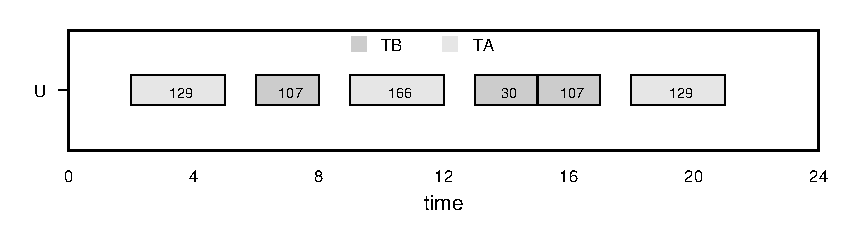
\includegraphics{SS_gantt.pdf}
\caption{Periodic production schedule to respond to nominal
  demands. The numbers indicate batch size}
\end{figure*}

\begin{figure*}
\begin{center}
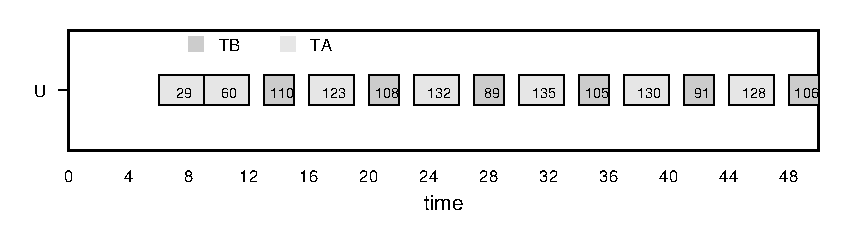
\includegraphics{NTS_gantt.pdf}
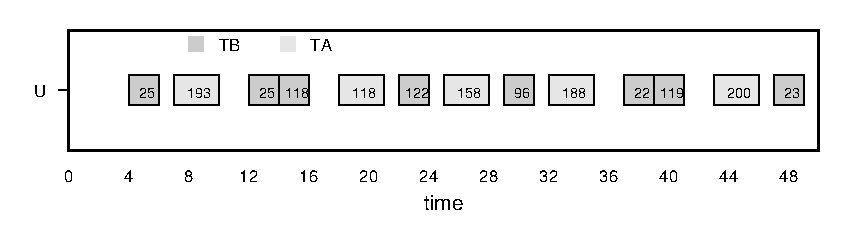
\includegraphics{TS_gantt.pdf}
\caption{Production schedule for the MPC without terminal constraints that optimized
  \eqref{eq:esc:PbNT} (Top) compared with production schedule for the MPC
  with terminal constraints that optimized \eqref{eq:esc:PbT}. Note how larger batches are made for
  the problem with terminal constraints}
\end{center}
\label{fig:abcdefg}
\end{figure*}

\begin{figure*}
\centering
\scriptsize
{\resizebox{1\textwidth}{!}{% GNUPLOT: LaTeX picture with Postscript
\begingroup
  \makeatletter
  \providecommand\color[2][]{%
    \GenericError{(gnuplot) \space\space\space\@spaces}{%
      Package color not loaded in conjunction with
      terminal option `colourtext'%
    }{See the gnuplot documentation for explanation.%
    }{Either use 'blacktext' in gnuplot or load the package
      color.sty in LaTeX.}%
    \renewcommand\color[2][]{}%
  }%
  \providecommand\includegraphics[2][]{%
    \GenericError{(gnuplot) \space\space\space\@spaces}{%
      Package graphicx or graphics not loaded%
    }{See the gnuplot documentation for explanation.%
    }{The gnuplot epslatex terminal needs graphicx.sty or graphics.sty.}%
    \renewcommand\includegraphics[2][]{}%
  }%
  \providecommand\rotatebox[2]{#2}%
  \@ifundefined{ifGPcolor}{%
    \newif\ifGPcolor
    \GPcolorfalse
  }{}%
  \@ifundefined{ifGPblacktext}{%
    \newif\ifGPblacktext
    \GPblacktexttrue
  }{}%
  % define a \g@addto@macro without @ in the name:
  \let\gplgaddtomacro\g@addto@macro
  % define empty templates for all commands taking text:
  \gdef\gplbacktext{}%
  \gdef\gplfronttext{}%
  \makeatother
  \ifGPblacktext
    % no textcolor at all
    \def\colorrgb#1{}%
    \def\colorgray#1{}%
  \else
    % gray or color?
    \ifGPcolor
      \def\colorrgb#1{\color[rgb]{#1}}%
      \def\colorgray#1{\color[gray]{#1}}%
      \expandafter\def\csname LTw\endcsname{\color{white}}%
      \expandafter\def\csname LTb\endcsname{\color{black}}%
      \expandafter\def\csname LTa\endcsname{\color{black}}%
      \expandafter\def\csname LT0\endcsname{\color[rgb]{1,0,0}}%
      \expandafter\def\csname LT1\endcsname{\color[rgb]{0,1,0}}%
      \expandafter\def\csname LT2\endcsname{\color[rgb]{0,0,1}}%
      \expandafter\def\csname LT3\endcsname{\color[rgb]{1,0,1}}%
      \expandafter\def\csname LT4\endcsname{\color[rgb]{0,1,1}}%
      \expandafter\def\csname LT5\endcsname{\color[rgb]{1,1,0}}%
      \expandafter\def\csname LT6\endcsname{\color[rgb]{0,0,0}}%
      \expandafter\def\csname LT7\endcsname{\color[rgb]{1,0.3,0}}%
      \expandafter\def\csname LT8\endcsname{\color[rgb]{0.5,0.5,0.5}}%
    \else
      % gray
      \def\colorrgb#1{\color{black}}%
      \def\colorgray#1{\color[gray]{#1}}%
      \expandafter\def\csname LTw\endcsname{\color{white}}%
      \expandafter\def\csname LTb\endcsname{\color{black}}%
      \expandafter\def\csname LTa\endcsname{\color{black}}%
      \expandafter\def\csname LT0\endcsname{\color{black}}%
      \expandafter\def\csname LT1\endcsname{\color{black}}%
      \expandafter\def\csname LT2\endcsname{\color{black}}%
      \expandafter\def\csname LT3\endcsname{\color{black}}%
      \expandafter\def\csname LT4\endcsname{\color{black}}%
      \expandafter\def\csname LT5\endcsname{\color{black}}%
      \expandafter\def\csname LT6\endcsname{\color{black}}%
      \expandafter\def\csname LT7\endcsname{\color{black}}%
      \expandafter\def\csname LT8\endcsname{\color{black}}%
    \fi
  \fi
  \setlength{\unitlength}{0.0500bp}%
  \begin{picture}(7200.00,3024.00)%
    \gplgaddtomacro\gplbacktext{%
      \csname LTb\endcsname%
      \put(946,802){\makebox(0,0)[r]{\strut{} 0}}%
      \put(946,1780){\makebox(0,0)[r]{\strut{} 50}}%
      \put(946,2759){\makebox(0,0)[r]{\strut{} 100}}%
      \put(1078,484){\makebox(0,0){\strut{} 0}}%
      \put(2223,484){\makebox(0,0){\strut{} 10}}%
      \put(3368,484){\makebox(0,0){\strut{} 20}}%
      \put(4513,484){\makebox(0,0){\strut{} 30}}%
      \put(5658,484){\makebox(0,0){\strut{} 40}}%
      \put(6803,484){\makebox(0,0){\strut{} 50}}%
      \put(176,1731){\rotatebox{-270}{\makebox(0,0){\strut{}Backorder -Retailer}}}%
      \put(3940,154){\makebox(0,0){\strut{}Time}}%
    }%
    \gplgaddtomacro\gplfronttext{%
      \csname LTb\endcsname%
      \put(5816,2586){\makebox(0,0)[r]{\strut{}Without terminal constraint}}%
      \csname LTb\endcsname%
      \put(5816,2366){\makebox(0,0)[r]{\strut{}With terminal constraint}}%
    }%
    \gplbacktext
    \put(0,0){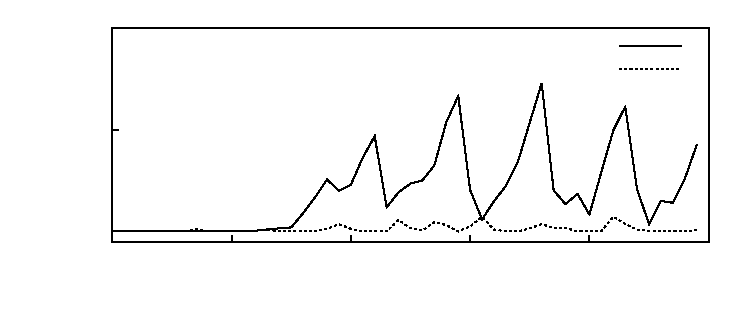
\includegraphics{BOprofile.pdf}}%
    \gplfronttext
  \end{picture}%
\endgroup
}}
\caption{Combined backorder at all the retailer nodes}
\label{fig:esc:BOTNT}
\end{figure*}
 Corresponding to Problem \eqref{eq:PN_none} and
 \eqref{eq:PN_equality}, we define the online MPC optimization problem
 without and with a periodic terminal
 constraint, respectively, as follows: 
 \begin{xalignat}{2}
\label{eq:esc:PbNT}
\mathbb{P}_N(x;\bd) :& \min_{\bu}{V_N(\bu;x)} & \nonumber \\
&\text{s.t.~} x(j+1) = Ax(j) + Bu(j) +B_dd(j), & j \in
\mathbb{I}_{0:N-1}\\
&(x(j),u(j))\in \mathbb{Z}& j \in \mathbb{I}_{0:N-1} \nonumber 
\end{xalignat}
\begin{xalignat}{2}
\label{eq:esc:PbT}
\mathbb{P}_N(x;\bd) :& \min_{\bu}{V_N(\bu;x)} & \nonumber \\
&\text{s.t.~} x(j+1) = Ax(j) + Bu(j) +B_dd(j), & j \in
\mathbb{I}_{0:N-1} \nonumber \\
&(x(j),u(j)) \in \mathbb{Z}& j \in \mathbb{I}_{0:N-1} \\
&x(N) \in \mathbb{X}_P & \nonumber
\end{xalignat}
in which $V_N(\bu;x)$ is the sum of the $N$ stages of economic cost $\ell_E(x,u)$. 

As shown in 
Figure \ref{fig:esc:BOTNT}, the solution to the simple re-optimization
of the $N$ period economic 
costs leads to greater backorders at the retailers. The backorders are
larger for the MPC without periodic constraint, 
\eqref{eq:esc:PbNT}, because the optimizer has no information
about the demands occurring after the planning period $N$. As a
result, it starts smaller batches (see Figure \ref{fig:abcdefg})
during the planning period. The cumulative effect of these decisions
is that there is not enough inventory when new demands are observed in
the subsequent optimization problems. On the other hand, in the MPC
with periodic constraint, \eqref{eq:esc:PbT},  the terminal constraint
$x(N) \in 
\mathbb{X}_P$ ensures that the decisions are made such that the supply
chain can respond to the nominal demand at the end of the planning
horizon. Hence, although, larger batches are started (see Figure
\ref{fig:abcdefg}), more inventory is
available to meet demands. Figure \ref{fig:esc:BOTNT} also highlights
the inherent robustness of the formulation \eqref{eq:esc:PbT}. It should
be noted that we have shown only convergence and not shown Lyapunov
stability for the MPC problem that solves \eqref{eq:esc:PbT}.  

\section{Conclusions}
\label{sec:conclusions}
The main contribution of this paper is to advance the research in
rolling horizon optimization framework for supply chain management by
demonstrating the design of model predictive control algorithms with
guaranteed closed-loop properties. We used recent developments in
economic MPC to design algorithms with guaranteed properties that
directly minimized the supply chain economics. We also proposed a
multiobjective cost function that captured the economics as well as
risk in the supply chain. The multiobjective cost function captures
the risk seeking/averse nature of the manager using a single
parameter. Finally, we demonstrated the integration of scheduling with
control on a multiechelon, multiproduct supply chain. We showed how a
properly chosen terminal constraint can add robustness to the rolling
horizon optimization framework. 

Among the directions for future research include: (a) developing new methods to
find terminal conditions for the integrated scheduling and control
problem; (b) applying existing and/or developing  new theory
for stability and convergence properties for the hybrid control problem,
and; (c) using demand forecasts and designing terminal
conditions for a robust demand scenario instead of a nominal demand
scenario. 

\paragraph{Acknowledgments}
This research is partially supported by the National Science Foundation
under Grant No. 0931835


\begin{thebibliography}{28}
\providecommand{\natexlab}[1]{#1}
\providecommand{\url}[1]{\texttt{#1}}
\expandafter\ifx\csname urlstyle\endcsname\relax
  \providecommand{\doi}[1]{doi: #1}\else
  \providecommand{\doi}{doi: \begingroup \urlstyle{rm}\Url}\fi

\bibitem[Amrit et~al.(2011)Amrit, Rawlings, and
  Angeli]{amrit:rawlings:angeli:2011}
R.~Amrit, J.~B. Rawlings, and D.~Angeli.
\newblock Economic optimization using model predictive control with a terminal
  cost.
\newblock \emph{Annual Rev. Control}, 35:\penalty0 178--186, 2011.

\bibitem[Braun et~al.(2003)Braun, Rivera, Flores, Carlyle, and
  Kempf]{braun:rivera:flores:carlyle:kempf:2003}
M.~Braun, D.~Rivera, M.~Flores, W.~Carlyle, and K.~Kempf.
\newblock A model predictive control framework for robust management of
  multi-product, multi-echelon demand networks.
\newblock \emph{Annual Reviews in Control}, 27\penalty0 (2):\penalty0 229--245,
  2003.

\bibitem[Diehl et~al.(2011)Diehl, Amrit, and
  Rawlings]{diehl:amrit:rawlings:2011}
M.~Diehl, R.~Amrit, and J.~B. Rawlings.
\newblock A {Lyapunov} function for economic optimizing model predictive
  control.
\newblock \emph{{IEEE} Trans. Auto. Cont.}, 56\penalty0 (3):\penalty0 703--707,
  2011.

\bibitem[Dunbar and Desa(2007)]{dunbar:desa:2007a}
W.~B. Dunbar and S.~Desa.
\newblock Distributed model predictive control for dynamic supply chain
  management.
\newblock In \emph{Assessment and Future Directions of Nonlinear Model
  Predictive Control}. Springer, 2007.

\bibitem[Gilbert and Tan(1991)]{gilbert:tan:1991}
E.~G. Gilbert and K.~T. Tan.
\newblock Linear systems with state and control constraints: {T}he theory and
  application of maximal output admissible sets.
\newblock \emph{{IEEE} Trans. Auto. Cont.}, 36\penalty0 (9):\penalty0
  1008--1020, September 1991.

\bibitem[Hoberg et~al.(2007)Hoberg, Bradley, and
  Thonemann]{hoberg:bradley:thonemann:2007}
K.~Hoberg, J.~R. Bradley, and U.~W. Thonemann.
\newblock Analyzing the effect of the inventory policy on order and inventory
  variability with linear control theory.
\newblock \emph{Eur. J. Oper. Res.}, 176\penalty0 (3):\penalty0 1620 -- 1642,
  2007.

\bibitem[Kempf(2004)]{kempf:2004}
K.~G. Kempf.
\newblock Control oriented approaches to supply chain management in
  semiconductor manufacturing.
\newblock In \emph{Proceedings of the 2004 American Control Conference}, July
  2004.

\bibitem[Kim and De~Weck(2005)]{kim:weck:2005}
I.~Kim and O.~De~Weck.
\newblock Adaptive weighted-sum method for bi-objective optimization: Pareto
  front generation.
\newblock \emph{Structural and Multidisciplinary Optimization}, 29\penalty0
  (2):\penalty0 149--158, 2005.

\bibitem[Kvasnica et~al.(2006)Kvasnica, Grieder, and
  Baoti\'{c}]{kvasnica:grieder:baotic:2006}
M.~Kvasnica, P.~Grieder, and M.~Baoti\'{c}.
\newblock \emph{{Multi-Parametric Toolbox (MPT)}}, 2006.
\newblock URL \url{http://control.ee.ethz.ch/~mpt/}.

\bibitem[Lee et~al.(1997{\natexlab{a}})Lee, Padmanabhan, and
  Whang]{lee:padmanabhan:whang:1997}
H.~L. Lee, V.~Padmanabhan, and S.~Whang.
\newblock The bullwhip effect in supply chains.
\newblock \emph{Sloan Manage. Rev.}, 38:\penalty0 93--102, 1997{\natexlab{a}}.

\bibitem[Lee et~al.(1997{\natexlab{b}})Lee, Padmanabhan, and
  Whang]{lee:padmanabhan:whang:1997b}
H.~L. Lee, V.~Padmanabhan, and S.~Whang.
\newblock Information distortion in a supply chain: The bullwhip effect.
\newblock \emph{Manage Sci.}, 43:\penalty0 546--558, 1997{\natexlab{b}}.

\bibitem[Lin et~al.(2004)Lin, Wong, Jang, Shieh, and
  Chu]{lin:wong:jang:shieh:chu:2004}
P.-H. Lin, D.~S.-H. Wong, S.-S. Jang, S.~S. Shieh, and J.-Z. Chu.
\newblock Controller design and reduction of bullwhip for a model supply chain
  system using z-transform analysis.
\newblock \emph{J. Proc. Cont.}, 14:\penalty0 487--499, September 2004.

\bibitem[Maestre et~al.(2009)Maestre, {D. Mu\~noz de la Pe\~na}, and
  Camacho]{Maestre:Pena:Camacho:2009}
J.~M. Maestre, {D. Mu\~noz de la Pe\~na}, and E.~F. Camacho.
\newblock Distributed {MPC}: {A} supply chain case study.
\newblock In \emph{Joint 48th {IEEE} Conference on Decision and Control and
  28th Chinese Control Conference}, 2009.

\bibitem[Maestre et~al.(2011)Maestre, {Mu\~noz de la Pe\~na}, and
  Camacho]{maestre:pena:camacho:2011}
J.~M. Maestre, D.~{Mu\~noz de la Pe\~na}, and E.~F. Camacho.
\newblock Distributed model predictive control based on a cooperative game.
\newblock \emph{Optimal Cont. Appl. Meth.}, 32\penalty0 (2):\penalty0 153--176,
  2011.

\bibitem[Maravelias(2012)]{maravelias:2012}
C.~Maravelias.
\newblock General framework and modeling approach classification for chemical
  production scheduling.
\newblock \emph{{AIChE} J.}, 2012.

\bibitem[M{\'e}ndez et~al.(2006)M{\'e}ndez, Cerd{\'a}, Grossmann, Harjunkoski,
  and Fahl]{mendez:cerda:grossmann:harjunkoski:fahl:2006}
C.~M{\'e}ndez, J.~Cerd{\'a}, I.~Grossmann, I.~Harjunkoski, and M.~Fahl.
\newblock State-of-the-art review of optimization methods for short-term
  scheduling of batch processes.
\newblock \emph{Comput. Chem. Eng.}, 30\penalty0 (6):\penalty0 913--946, 2006.

\bibitem[Mestan et~al.(2006)Mestan, T{\"u}rkay, and
  Arkun]{mestan:turkay:arkun:2006}
E.~Mestan, M.~T{\"u}rkay, and Y.~Arkun.
\newblock Optimization of operations in supply chain systems using hybrid
  systems approach and model predictive control.
\newblock \emph{Ind. Eng. Chem. Res.}, 45:\penalty0 6493--6503, August 2006.

\bibitem[Moyaux et~al.(2007)Moyaux, Chain-draa, and
  D'Amours]{moyaux:chaib-draa:damours:2007}
T.~Moyaux, B.~Chain-draa, and S.~D'Amours.
\newblock Information sharing as a coordination mechanism for reducing the
  bullwhip effect in a supply chain.
\newblock \emph{{IEEE} T. Syst. Man Cy. C}, 37\penalty0 (3):\penalty0 396--409,
  2007.

\bibitem[Ortega and Lin(2004)]{ortega:lin:2004}
M.~Ortega and L.~Lin.
\newblock Control theory applications to the production--inventory problem: {A}
  review.
\newblock \emph{Int. J. Prod. Res.}, 42:\penalty0 2303--2322, 2004.

\bibitem[Perea~L{\'o}pez et~al.(2003)Perea~L{\'o}pez, Ydstie, and
  Grossmann]{perealopez:ydstie:grossmann:2003}
E.~Perea~L{\'o}pez, B.~E. Ydstie, and I.~E. Grossmann.
\newblock A model predictive control strategy for supply chain optimization.
\newblock \emph{Comput. Chem. Eng.}, 27\penalty0 (8-9):\penalty0 1201--1218,
  February 2003.

\bibitem[Rao and Rawlings(1999)]{rao:rawlings:1999}
C.~V. Rao and J.~B. Rawlings.
\newblock Steady states and constraints in model predictive control.
\newblock \emph{{AIChE} J.}, 45\penalty0 (6):\penalty0 1266--1278, 1999.

\bibitem[Rawlings and Mayne(2009)]{rawlings:mayne:2009}
J.~B. Rawlings and D.~Q. Mayne.
\newblock \emph{Model Predictive Control: Theory and Design}.
\newblock Nob Hill Publishing, Madison, WI, 2009.
\newblock 576 pages, ISBN 978-0-9759377-0-9.

\bibitem[Sarimveis et~al.(2008)Sarimveis, Patrinos, Tarantilis, and
  Kiranoudis]{sarimevis:patrinos:tarantilis:kiranoudis:2008}
H.~Sarimveis, P.~Patrinos, C.~D. Tarantilis, and C.~T. Kiranoudis.
\newblock Dynamic modeling and control of supply chains: {A} review.
\newblock \emph{Comput. Oper. Res.}, 35:\penalty0 3530--3561, 2008.

\bibitem[Seferlis and Giannelos(2004)]{seferlis:giannelos:2004}
P.~Seferlis and N.~F. Giannelos.
\newblock A two-layered optimization-based control strategy for multi-echelon
  supply chain networks.
\newblock \emph{Comput. Chem. Eng.}, 28:\penalty0 1121--1129, 2004.

\bibitem[Shah et~al.(1993)Shah, Pantelides, and
  Sargent]{shah:pantelides:sargent:1993}
N.~Shah, C.~C. Pantelides, and R.~Sargent.
\newblock A general algorithm for short term scheduling of batch
  operations--{II}. {C}omputational issues.
\newblock \emph{Comput. Chem. Eng.}, 20:\penalty0 229--244, 1993.

\bibitem[Subramanian et~al.(2012)Subramanian, Maravelias, and
  Rawlings]{subramanian:maravelias:rawlings:2012}
K.~Subramanian, C.~T. Maravelias, and J.~B. Rawlings.
\newblock A state-space model for chemical production scheduling.
\newblock \emph{Comput. Chem. Eng.}, 47:\penalty0 97--110, December 2012.

\bibitem[Subramanian et~al.(2013)Subramanian, Rawlings, and
  Maravelias]{subramanian:rawlings:maravelias:2013}
K.~Subramanian, J.~B. Rawlings, and C.~T. Maravelias.
\newblock Integration of control theory and scheduling methods for supply chain
  management.
\newblock \emph{Comput. Chem. Eng.}, 51:\penalty0 4--20, April 2013.

\bibitem[Venkateswaran and Son(2005)]{venkateswaran:son:2005}
J.~Venkateswaran and Y.~J. Son.
\newblock Information synchronization effects on the stability of collaborative
  supply chain.
\newblock In \emph{Simulation Conference Proceedings, 2005. Winter}, pages
  1668--1676, 2005.

\end{thebibliography}
\end{document}

